%\documentclass[spanish,a4paper,11pt,oneside,links]{report}
\documentclass[spanish,a4paper,oneside,10pt,openright]{book}
\usepackage[T1]{fontenc}
\usepackage{graphicx}
\usepackage{amsmath,amsfonts,amssymb}
\usepackage[utf8]{inputenc}
\usepackage[spanish, es-tabla]{babel}
\usepackage[Algoritmo]{algorithm}
\usepackage{algpseudocode}
\usepackage{url}
\usepackage{fancyhdr}
\usepackage{epstopdf}
\usepackage{minted}
    \setminted{
        autogobble,
        breaklines=true,
        linenos=true,
    }
    \usemintedstyle{pastie}
\usepackage{csquotes}
\usepackage{rotating}
\usepackage{zref-xr}
\usepackage{amssymb}
\usepackage[pdfencoding=auto, psdextra]{hyperref}
\usepackage{multicol}
\usepackage{spverbatim}
\usepackage[pdf]{graphviz}
\usepackage{dirtree}
\usepackage{tabularx}
    \newcolumntype{L}{>{\raggedright\arraybackslash}X}
\usepackage{emptypage}
\usepackage[acronym,toc,shortcuts,xindy]{glossaries}
\usepackage{markdown}
\usepackage{booktabs}
\usepackage{xcolor}
\usepackage{changepage}
\usepackage{tcolorbox}
\usepackage{siunitx}
\usepackage{bold-extra}
\usepackage[backend=biber,style=apa,natbib=true]{biblatex}
\usepackage{svg}
\usepackage{morewrites}
\usepackage{aas_macros}
\usepackage{caption}
\usepackage{subcaption}
\usepackage{enumitem}
\usepackage{float}
\usepackage{floatpag}
\usepackage{lipsum}

%%%%% GLOSSARY START
% Add new key for long Spanish form:
\glsaddkey
{longsp}% key
{}% default value
{\glsentrylongsp}% new command analogous to \glsentrylong
{\Glsentrylongsp}% new command analogous to \Glsentrylong
{\acrlongsp}% new command analogous to \acrlong
{\Acrlongsp}% new command analogous to \Acrlong
{\ACRlongsp}% new command analogous to \ACRlong

% Add new key for plural long Spanish form:
\glsaddkey
{longplsp}% key
{}% default value
{\glsentrylongplsp}% new command analogous to \glsentrylongpl
{\Glsentrylongplsp}% new command analogous to \Glsentrylongpl
{\acrlongplsp}% new command analogous to \acrlongpl
{\Acrlongplsp}% new command analogous to \Acrlongpl
{\ACRlongplsp}% new command analogous to \ACRlongpl

% Provide conditional to test if longsp/longplsp has been set
\newcommand*{\glsifhaslongsp}[3]{%
  \ifcsempty{glo@#1@longsp}{#3}{#2}%
}
\newcommand*{\glsifhaslongplsp}[3]{%
  \ifcsempty{glo@#1@longplsp}{#3}{#2}%
}

% Define new acronym style:

\newacronymstyle{spanish}
{% base the display style on 'long-short'
  \GlsUseAcrEntryDispStyle{long-short}%
}%
{% base the definitions on 'long-short'
  \GlsUseAcrStyleDefs{long-short}%  
% Make some custom modifications for the first use display.
% Singular, no case change:
  \renewcommand*{\genacrfullformat}[2]{%
   \glsifhaslongsp{##1}%
   {% has Spanish version:
      \glsentrylongsp{##1}##2\space
      (\firstacronymfont{\glsentryshort{##1}}, \glsentrylong{##1})%
   }%
   {%
     \glsentrylong{##1}##2\space
     (\firstacronymfont{\glsentryshort{##1}})%
   }%
  }%
% Singular, first letter upper case:
  \renewcommand*{\Genacrfullformat}[2]{%
   \glsifhaslongsp{##1}%
   {% has Spanish version:
      \Glsentrylongsp{##1}##2\space
      (\firstacronymfont{\glsentryshort{##1}}, \glsentrylong{##1})%
   }%
   {%
     \Glsentrylong{##1}##2\space
     (\firstacronymfont{\glsentryshort{##1}})%
   }%
  }%
% Plural, no case change:
  \renewcommand*{\genplacrfullformat}[2]{%
   \glsifhaslongplsp{##1}%
   {% has Spanish version:
      \glsentrylongplsp{##1}##2\space
      (\firstacronymfont{\glsentryshortpl{##1}}, \glsentrylongpl{##1})%
   }%
   {%
     \glsentrylongpl{##1}##2\space
     (\firstacronymfont{\glsentryshortpl{##1}})%
   }%
  }%
% Plural, first letter upper case:
  \renewcommand*{\Genplacrfullformat}[2]{%
    \glsifhaslongplsp{##1}%
    {% has Spanish version:
      \Glsentrylongplsp{##1}##2\space
      (\firstacronymfont{\glsentryshortpl{##1}}, \glsentrylongpl{##1})%
    }%
    {%
      \Glsentrylongpl{##1}##2\space
      (\firstacronymfont{\glsentryshortpl{##1}})%
    }%
  }%
}

% switch to the new style:
\setacronymstyle{spanish}

% Define a new glossary style that checks for the existence of
% the longsp field.
\newglossarystyle{listsp}{%
  \setglossarystyle{list}% base style on the list style
  \renewcommand*{\glossentry}[2]{%
  \item[\glsentryitem{##1}%
        \glstarget{##1}{\glossentryname{##1}}]
    \glossentrydesc{##1}%
    \glsifhaslongsp{##1}{\space(\glsentrylongsp{##1})}{}%
    \glspostdescription\space ##2}%
}
%%%%% GLOSSARY END


\addbibresource{tesis.bib} % Imports bibliography file

% wide page for side by side figures, tables, etc
\newlength{\offsetpage}
\setlength{\offsetpage}{1.0cm}
\newenvironment{widepage}{\begin{adjustwidth}{-\offsetpage}{-\offsetpage}%
    \addtolength{\textwidth}{2\offsetpage}}%
{\end{adjustwidth}}

\newtheorem{definition}{Definición}

\renewcommand{\listalgorithmname}{Índice de Algoritmos}

\newenvironment{code}{\captionsetup{type=listing}}{}



\DeclareMathOperator*{\argmax}{arg\,max}  % in your preamble
\DeclareMathOperator*{\argmin}{arg\,min}  % in your preamble

\makeglossaries

\newacronym[longsp=curva de luz, longplsp=curvas de luz, shortplural={LCs}]{lc}{LC}{\emph{Light Curve}}
\newacronym[longsp=día juliano, longplsp=días julianos, shortplural={JD}]{jd}{JD}{\emph{Julian Day}}
\newacronym{feets}{feets}{\emph{feATURE eXTRACTOR FOR tIME sERIES}}
\newacronym{fats}{FATS}{\emph{Feature Extraction for Time Series}}
\newacronym{vista}{VISTA}{\emph{Visible and Infrared Survey Telescope for Astronomy}}
\newacronym{vvv}{VVV}{\emph{\acrshort{vista} Variables in the Via Lactea}}
\newacronym{vvvx}{VVVX}{\emph{\acrshort{vvv} eXtended}}
\newacronym[longsp=aprendizaje automático]{ml}{ML}{\emph{Machine Learning}}
\newacronym[longsp=minería de datos]{dm}{DM}{\emph{Data Mining}}
\newacronym[longsp=descubrimiento de conocimiento en bases de datos]{kdd}{KDD}{\emph{Knowledge Discovery in Databases}}
\newacronym[longsp=interfaz abstracta de programación, longplsp=interfaces abstractas de programación]{api}{API}{\emph{Application Programming Interface}}
\newacronym[longsp=complejidad ciclomática]{cc}{CC}{\emph{Cyclomatic Complexity}}
\newacronym{hv}{V}{volumen de Halstead}
\newacronym[longsp=líneas de código]{loc}{LOC}{\emph{Lines Of Code}}
\newacronym[longsp=porcentaje de comentarios]{poc}{POC}{\emph{Percentage Of Comments}}
\newacronym[longsp=índice de mantenibilidad]{mi}{MI}{\emph{Maintainability Index}}
\newacronym{gil}{GIL}{\emph{Global Interpreter Lock}}
\newacronym{ogle}{OGLE-III}{\emph{Optical Gravitational Lensing Experiment}}
\newacronym{macho}{MACHO}{\emph{Massive Compact Halo Objects}}
\newacronym{unc}{UNC}{Universidad Nacional de Córdoba}
\newacronym{sei}{SEI}{\emph{Software Engineering Institute}}

% \newacronym
%  [longsp=interfaz de programaci\'{o}n de la aplicaci\'{o}n,
%   longplsp=interfaces de programaci\'{o}n de la aplicaci\'{o}n
%  ]{api}{API}{Application Programming Interface}

% \newacronym{aa}{AA}{Another Acronym}

\lhead[]{\rightmark}
\chead[]{}
\rhead[\leftmark]{}
\renewcommand{\headrulewidth}{0.5pt}

\fancypagestyle{plain}{
\fancyhead[L]{}
\fancyhead[C]{}
\fancyhead[R]{}
\renewcommand{\headrulewidth}{0pt}
}

\pagestyle{fancy}

\widowpenalty 10000
\clubpenalty 10000

\setlength{\headheight}{25.07225pt}


% AGREGAGO POR JUAN =====================================================
% COMANDOS DE CORRECCION
\newcommand{\authorname}{{Felipe Clariá Dambolena}}
\newcommand{\unc}{{Universidad Nacional de Córdoba}}
\newcommand{\jbc}[1]{{\color{olive} #1 (JBC)\ }}
\newcommand{\citeme}[1]{{\color{red}{¡¡CITEME: #1!!}}}
\newcommand{\todo}[1]{{\color{red!75}{Completar: #1}}}

% SNIPPETS DE CODIGO
\providecommand*{\listingautorefname}{Código}
\renewcommand{\listingscaption}{Código}
\renewcommand{\thelisting}{\thesection.\arabic{listing}}
\usepackage{etoolbox}
\renewcommand{\thelisting}{\thesection.\arabic{listing}}
\preto\section{\setcounter{listing}{0}}


\begin{document}

\begin{titlepage}

% Configuración del espaciado
% \setstretch{1.5}

% LOGOS SUPERIORES
\noindent
\begin{figure}[!ht]
\centering
\begin{subfigure}{0.5\textwidth}
    \flushleft
    
\includegraphics[width=5cm]{00_tapa/figures/logo_unc.png}
\end{subfigure}%
\begin{subfigure}{0.5\textwidth}
    \flushright
    
\includegraphics[width=5cm]{00_tapa/figures/logo_famaf.png}
\end{subfigure}
\end{figure}

\vspace{2.5cm}

% TÍTULO Y AUTOR
\begin{center}
    {\huge Optimización y paralelización de cómputo para extracción de características de estrellas variables periódicas} \\ [0.5cm]
    {\Large por} \\
    {\Large \authorname}
\end{center}

\vspace{1.5cm} 

% TEXTO DESCRIPTIVO
\noindent
Presentado ante la FACULTAD DE MATEMÁTICA, ASTRONOMÍA, FÍSICA Y COMPUTACIÓN como parte de los requerimientos para la obtención del grado de Licenciado en Ciencias de la Computación de la

\begin{center}
    UNIVERSIDAD NACIONAL DE CÓRDOBA
\end{center}

\vspace{1cm}

\noindent
\begin{center}
    Mayo, 2025
\end{center}

\vspace{0.5cm}

% DIRECTOR/A
\noindent
\begin{center}
{\large Directores: Dr. Juan B. Cabral \\ Dr. Bruno O. Sanchez}
\end{center}

\vfill % Espacio hasta el final de la página

% LICENCIA CREATIVE COMMONS
\begin{center}
    
\includegraphics[width=2cm]{00_tapa/figures/by-sa.png}\\    \vspace{0.3cm}
      {\small Optimización y paralelización de cómputo para extracción de características de estrellas variables periódicas © 2025 by Felipe Clariá is licensed under Creative Commons Attribution-ShareAlike 4.0 International. To view a copy of this license, visit \url{https://creativecommons.org/licenses/by-sa/4.0/}}
\end{center}

\end{titlepage}
 \cleardoublepage


\pagenumbering{gobble}
Certifico que el trabajo incluido en este documento es el resultado de tareas de investigación originales y que no ha sido presentado para optar a un título de posgrado en ninguna otra Universidad o Institución.

\vspace{3cm}
\begin{flushright}
\authorname
\end{flushright}
\cleardoublepage

% RECONOCIMIENTS + AGRADECIMIENTOS ============================================

\phantom{p. 1}
\thispagestyle{empty}

\chapter*{Reconocimientos}
\pagenumbering{Roman} % para comenzar la numeracion de paginas en numeros romanos
\addcontentsline{toc}{chapter}{Reconocimientos} % si queremos que aparezca en el índice
\markboth{RECONOCIMIENTOS}{RECONOCIMIENTOS} % encabezado
Este trabajo utilizó recursos computacionales de UNC Supercómputo (CCAD) de la \unc \footnote{\url{https://supercomputo.unc.edu.ar}}, que forman parte del Sistema Nacional de Computación de Alto Desempeño (SNCAD) de la República Argentina.

\phantom{p. 1}
\clearpage
\thispagestyle{empty}
\phantom{p. 2}
\clearpage

\chapter*{Agradecimientos} % si no queremos que añada la palabra "Capitulo"
% \pagenumbering{Roman} % para comenzar la numeracion de paginas en numeros romanos
\addcontentsline{toc}{chapter}{Agradecimientos} % si queremos que aparezca en el índice
\markboth{AGRADECIMIENTOS}{AGRADECIMIENTOS} % encabezado
Quiero expresar mi profundo agradecimiento a mis directores, el Dr. Juan Bautista Cabral y el Dr. Bruno O. Sánchez, por su constante disposición, guía y compromiso a lo largo de todo el desarrollo de este trabajo. Su acompañamiento fue fundamental tanto en los aspectos técnicos como en los momentos de duda o incertidumbre.

Agradezco también a la \unc{} por brindarme una formación académica de excelencia, y en particular a la Facultad de Matemática, Astronomía, Física y Computación por ofrecerme un espacio de estudio, crecimiento y pertenencia durante toda mi carrera. Tanto la institución como su comunidad fueron pilares en mi desarrollo académico y personal.

A mi familia, especialmente a mi madre Eugenia y a mi padre Carlos, por su amor, su apoyo incondicional y por sostenerme durante todos estos años. A mis hermanos Lucía y Julián, por estar siempre cerca, y a mis mascotas, Prim, Pepé, Betty y Tofi.

A mis compañeros de ruta en este tramo final de la carrera, Gino, Álvaro y Diego. Su compañía, apoyo y motivación constantes fueron de gran ayuda durante todo este proceso.

A mis amigos de la vida, Matteo, Agustín, Jazmín y Clarita, por estar presentes, por su cariño, y por ser parte esencial de mi bienestar emocional. Los quiero con todo mi corazón.

Finalmente, agradezco también a quien se tome el tiempo de leer este trabajo. Espero que encuentre en estas páginas un aporte valioso y bien intencionado, fruto de mucho esfuerzo y dedicación.

% ABSTRACT ====================================================================

\phantom{p. 1}
\clearpage
\thispagestyle{empty}
\phantom{p. 2}
\clearpage

\chapter*{Resumen} % si no queremos que añada la palabra "Capitulo"
\addcontentsline{toc}{chapter}{Resumen} % si queremos que aparezca en el índice
\markboth{RESUMEN}{RESUMEN} % encabezado
El crecimiento exponencial de los datos astronómicos ha planteado nuevos desafíos en el análisis eficiente de curvas de luz, fundamentales para el estudio de estrellas variables periódicas. Este trabajo aborda la optimización y modernización de la biblioteca \acrfull{feets}, una herramienta de Python para la extracción de características de curvas de luz. Presentamos una refactorización integral que incorpora una nueva implementación paralela que busca reducir los tiempos de cómputo, con un rediseño arquitectónico basado en principios de ingeniería de \emph{software}. Los resultados obtenidos demuestran una reducción notable en los tiempos de ejecución y una mejora sustancial en la calidad del código, lo que posiciona a la nueva versión de \acrshort{feets} como una herramienta escalable para el análisis astronómico de grandes volúmenes de datos.

\phantom{p. 1}
\clearpage
\thispagestyle{empty}

\chapter*{Abstract} % si no queremos que añada la palabra "Capitulo"
\addcontentsline{toc}{chapter}{Abstract} % si queremos que aparezca en el índice
\markboth{ABSTRACT}{ABSTRACT} % encabezado
The exponential growth of astronomical data has posed new challenges in the efficient analysis of light curves, fundamental to the study of periodic variable stars. This work addresses the optimization and modernization of the \acrfull{feets} library, a Python tool for light curve feature extraction. We present a comprehensive refactoring incorporating a new parallel implementation that aims to reduce computational time, with an architectural redesign based on software engineering principles. The results demonstrate a notable reduction in execution time and a substantial improvement in code quality, positioning the new version of \acrshort{feets} as a scalable tool for astronomical analysis of large volumes of data.

\phantom{p. 1}
\thispagestyle{empty}


% GLOSARIO=====================================================================

\renewcommand*\glspostdescription{\dotfill}
\setlength{\glslistdottedwidth}{1\textwidth}
\setlength{\glsdescwidth}{0.89\textwidth}
\markboth{Glosario}{Glosario} % encabezado
\glsaddall
\printglossary[type=\acronymtype,title=Glosario]
\addcontentsline{toc}{chapter}{Glosario}


% CONTENIDOS ==================================================================
\phantom{p. 1}
\clearpage

\tableofcontents % indice de contenidos

\phantom{p. 1}
\thispagestyle{empty}

% FIGURES =====================================================================

\cleardoublepage
\listoffigures % indice de figuras
\addcontentsline{toc}{chapter}{Índice de figuras} % para que aparezca en el indice de contenidos

% \phantom{p. 1}
% \thispagestyle{empty}
% \phantom{p. 1}
% \clearpage

% %%%%

% \phantom{p. 1}
% \clearpage
% \thispagestyle{empty}
% \phantom{p. 2}
% \clearpage

% \chapter*{Resumen} % si no queremos que añada la palabra "Capitulo"
% \addcontentsline{toc}{chapter}{Resumen} % si queremos que aparezca en el índice
% \markboth{RESUMEN}{RESUMEN} % encabezado
% El crecimiento exponencial de los datos astronómicos ha planteado nuevos desafíos en el análisis eficiente de curvas de luz, fundamentales para el estudio de estrellas variables periódicas. Este trabajo aborda la optimización y modernización de la biblioteca \acrfull{feets}, una herramienta de Python para la extracción de características de curvas de luz. Presentamos una refactorización integral que incorpora una nueva implementación paralela que busca reducir los tiempos de cómputo, con un rediseño arquitectónico basado en principios de ingeniería de \emph{software}. Los resultados obtenidos demuestran una reducción notable en los tiempos de ejecución y una mejora sustancial en la calidad del código, lo que posiciona a la nueva versión de \acrshort{feets} como una herramienta escalable para el análisis astronómico de grandes volúmenes de datos.

% \phantom{p. 1}
% \clearpage
% \thispagestyle{empty}

% \chapter*{Abstract} % si no queremos que añada la palabra "Capitulo"
% \addcontentsline{toc}{chapter}{Abstract} % si queremos que aparezca en el índice
% \markboth{ABSTRACT}{ABSTRACT} % encabezado
% The exponential growth of astronomical data has posed new challenges in the efficient analysis of light curves, fundamental to the study of periodic variable stars. This work addresses the optimization and modernization of the \acrfull{feets} library, a Python tool for light curve feature extraction. We present a comprehensive refactoring incorporating a new parallel implementation that aims to reduce computational time, with an architectural redesign based on software engineering principles. The results demonstrate a notable reduction in execution time and a substantial improvement in code quality, positioning the new version of \acrshort{feets} as a scalable tool for astronomical analysis of large volumes of data.

% \phantom{p. 1}
% \thispagestyle{empty}

% TABLES ======================================================================

% \cleardoublepage
% \listoftables % indice de tablas
% \addcontentsline{toc}{chapter}{Índice de tablas} % para que aparezca en el indice de contenidos

% % pagina en blanco
% \newpage

\phantom{p. 1}
\clearpage
\pagenumbering{arabic}


% CONTENT =====================================================================

\chapter{Introducción}
\label{chapter:intro}
El desarrollo de modernos telescopios y satélites ha posibilitado la realización de relevamientos astronómicos a una escala sin precedentes, lo que ha generado un aumento exponencial tanto en la cantidad como en la calidad de los datos disponibles para su procesamiento, almacenamiento y análisis \citep{cavuoti2013datarichastronomyminingsynoptic}. Entre ellos, el relevamiento \gls{vvv} llevó a cabo un censo exhaustivo de estrellas en el disco y bulbo galáctico durante un período de cinco años \citep{minniti2010vvv}, utilizando el telescopio infrarrojo \gls{vista}, ubicado en el Cerro Paranal, Chile.

El \gls{vvv} produjo un volumen de datos superior a los $\SI{300}{\giga\byte}$ por noche, organizados en unidades de observación denominadas \emph{tiles}, que corresponden a áreas rectangulares del cielo observadas repetidamente. Cada observación incluye imágenes de alta resolución en distintos filtros lumínicos, junto con catálogos fotométricos que contienen información detallada sobre las fuentes de luz detectadas, como posición, magnitud y color. Estos catálogos son fundamentales para tareas como la construcción de mapas tridimensionales del entorno observado. En particular, la identificación de estrellas variables periódicas resulta esencial, ya que estas funcionan como indicadores precisos de distancia.

Frente a volúmenes de datos tan extensos como los del \gls{vvv}, las técnicas de \gls{ml} se han consolidado como herramientas indispensables para automatizar la detección, clasificación y análisis de objetos de interés \citep{Bai_2018, Cabral_2020, Ye_2019}. Una etapa crítica en estos flujos de trabajo es la extracción de características a partir de \acrfullpl{lc}, entendidas como series temporales que registran la evolución del brillo de una fuente en función del tiempo. Este proceso permite transformar los datos crudos en representaciones más significativas y adecuadas para alimentar modelos de \gls{ml}, pero representa una tarea intensiva en recursos computacionales, especialmente cuando trabajamos con millones de curvas provenientes de relevamientos extensos.

Herramientas como \acrfull{feets} han demostrado ser útiles al automatizar el cálculo de decenas de características diseñadas específicamente para el análisis de series temporales astronómicas \citep{cabral2018feets}. La biblioteca, desarrollada en Python, proporciona un conjunto modular de extractores de características capaces de obtener métricas estadísticas, propiedades de variabilidad y medidas periódicas a partir de un conjunto de vectores representativos de una \gls{lc}.

La versión original de \gls{feets} realiza todos los cálculos de forma secuencial, evaluando uno por uno cada extractor sobre la curva de entrada. Este enfoque impone un cuello de botella significativo cuando necesitamos procesar grandes volúmenes de datos: en un escenario realista como el del \gls{vvv}, procesar el conjunto completo de \emph{tiles} podría demorar entre ocho meses y dos años y medio, considerando que cada \emph{tile} contiene en promedio más de 100 mil fuentes.

En este trabajo presentamos una refactorización  \citep{fowler1999refactoring} completa de \gls{feets} para adaptarla a los desafíos actuales del análisis astronómico, enfocándonos en su paralelización, la modernización de su entorno tecnológico y el rediseño de su arquitectura interna. La nueva versión implementa un modelo de extracción paralelizado, con estrategias de \emph{multiprocessing} \citep{baer1976multiprocessing}, que mejora significativamente la escalabilidad y los tiempos de cómputo, y adopta tecnologías actuales para optimizar el rendimiento. Además, rediseñamos la interfaz de la aplicación y simplificamos el \emph{framework} para la creación de extractores, incorporando nuevas funcionalidades y principios de diseño de \emph{software} orientados a mejorar la mantenibilidad y extensibilidad del sistema.

El resultado es una nueva versión de \gls{feets} moderna, robusta y escalable, capaz de afrontar los retos computacionales de la astronomía observacional sin comprometer la calidad del software.

\section{Organización del trabajo}

Los capítulos de este trabajo se organizan de la siguiente manera:

En el \autoref{chapter:antecedentes} se presentan los fundamentos astronómicos, computacionales y de diseño de software que sirven de base para este trabajo. Se describe el papel de las \gls{lc} y las técnicas de \gls{ml} aplicadas al análisis astronómico. También se abordan conceptos clave sobre calidad de software y de cómputo distribuido. 

El \autoref{chapter:feets} describe el estado de \gls{feets}, detallando las funcionalidades, la arquitectura y las limitaciones presentes en el código original. 

Los Capítulos~\ref{chapter:parallel} y~\ref{chapter:refactoring} documentan el desarrollo de la nueva versión de \gls{feets}. Abordan la implementación del nuevo modelo de extracción paralelizado y el proceso de modernización y refactorización general de la herramienta, respectivamente.

En el \autoref{chapter:resultados} se presentan los resultados obtenidos en la nueva versión, tanto en términos de rendimiento como de calidad del código.

Finalmente, las conclusiones generales del trabajo son presentadas en el \autoref{chapter:conclusiones}, donde también se discuten posibles líneas futuras de desarrollo.


 \cleardoublepage
\chapter{Antecedentes y estado del arte}
\label{chapter:antecedentes}

\section{Las estrellas variables y el cosmos}

El análisis fotométrico de estrellas variables ha transformado nuestro entendimiento del universo. Gracias a su utilidad en la medición de distancias cósmicas, han permitido estimar las dimensiones de nuestra galaxia \citep{shapley1917stellarclusters} y confirmar la existencia de otros ``universos isla'' más allá de la Vía Láctea \citep{hubble1925cepheids}. Además, han proporcionado una base sólida  en la determinación de parámetros cosmológicos fundamentales, como la constante de Hubble \citep{freedman2001hubble, riess1998acceleration}, lo que llevó al descubrimiento de la expansión acelerada del universo. Su estudio también ha contribuido al entendimiento de la evolución estelar \citep{eddington1919gaseousstar} y los procesos de formación planetaria \citep{menard2002disks}, entre otros aportes.

Las estrellas variables son aquellas cuyo brillo, tal como se lo observa desde la Tierra, experimenta cambios a lo largo del tiempo. Estas variaciones pueden ser de diversa intensidad y ocurrir en escalas temporales que van desde milisegundos hasta décadas. La clasificación de las estrellas variables típicamente se basa en las causas subyacentes de sus variaciones de brillo \citep{eyer2008hr}. Como se observa en la \autoref{fig:classification}, se pueden distinguir dos grandes grupos: las estrellas extrínsecas y las intrínsecas.

\begin{figure}[!ht]
    \centering
    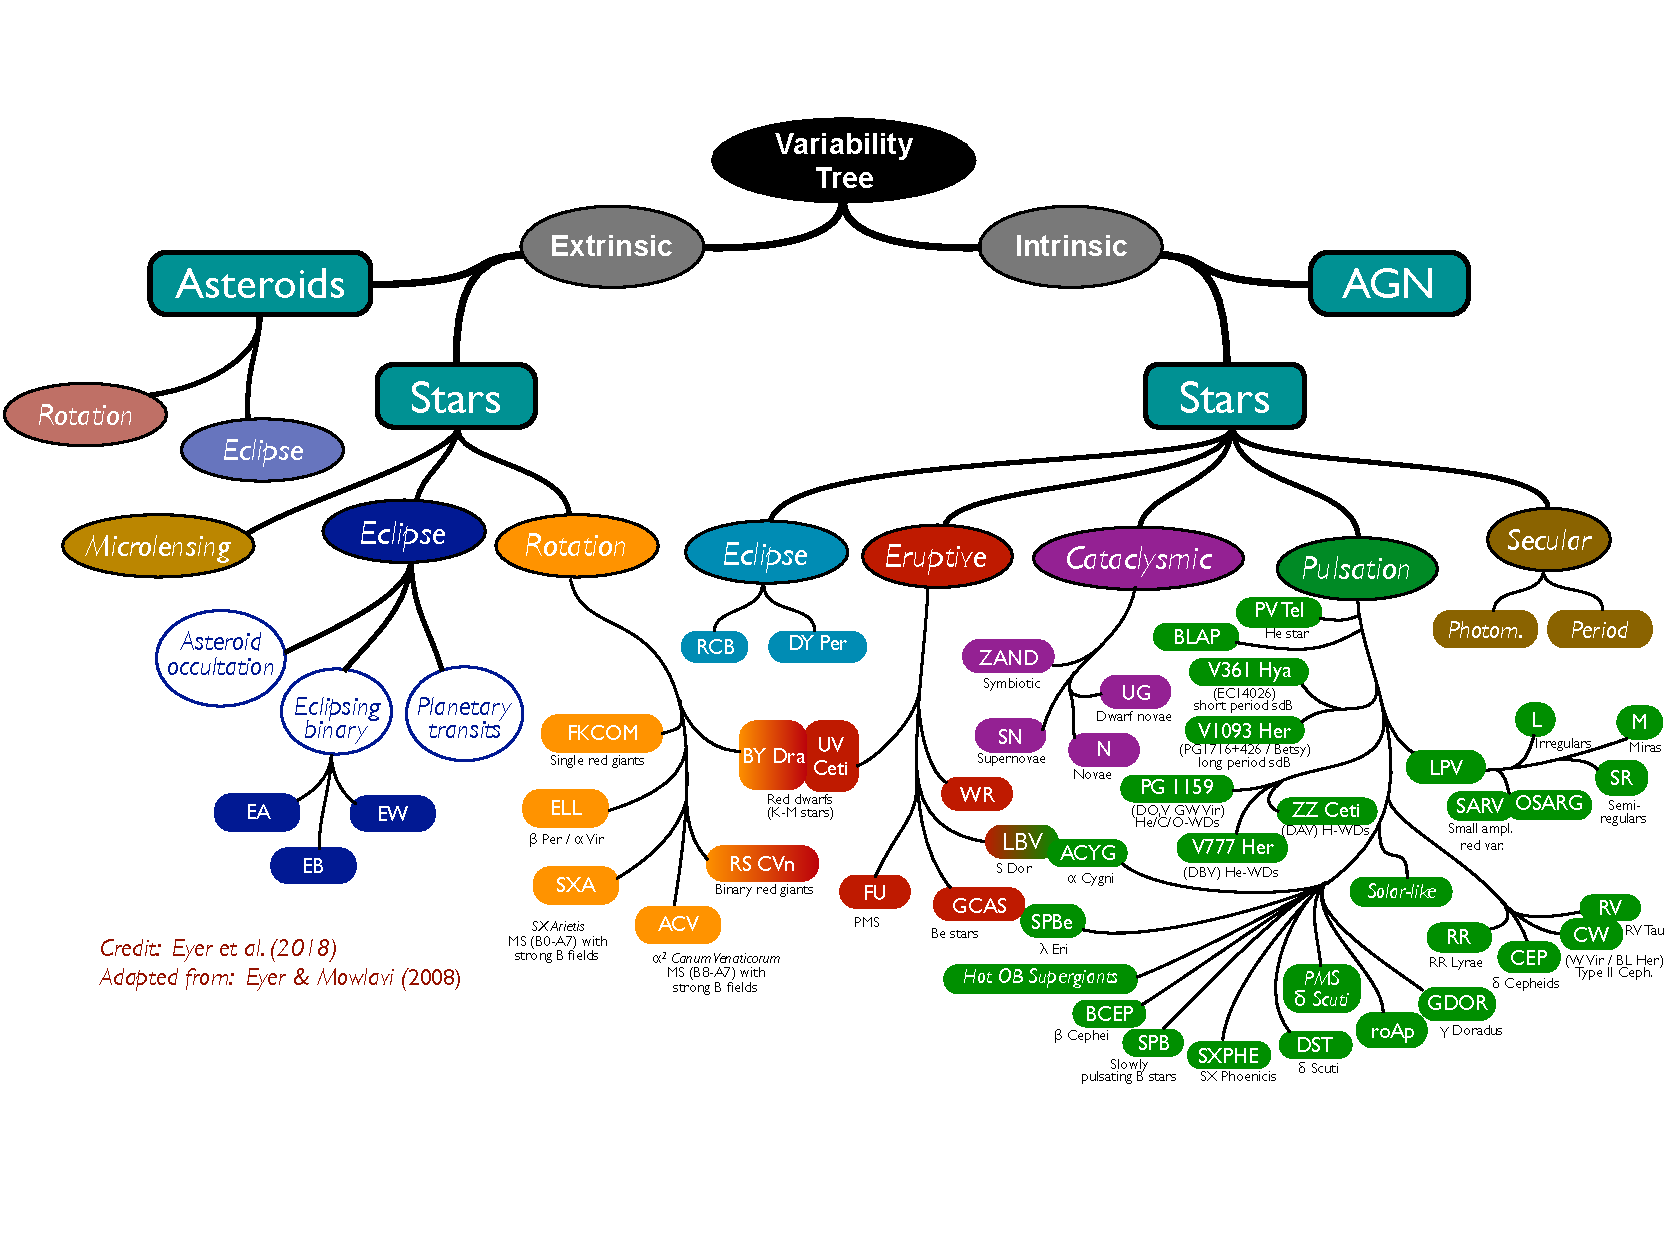
\includegraphics[width=1\linewidth]{04_antecedentes/figures/classification.pdf}
    \caption{
       Árbol de variabilidad. Expone en detalle la organización de objetos variables. Crédito: \citet{eyer2019gaia}. 
    }
    \label{fig:classification}
\end{figure}

En las variables extrínsecas, los cambios de brillo son el producto de ocurrencias externas, como pueden ser las interacciones de la estrella con otros cuerpos celestes o los efectos de su rotación estelar. Un caso característico de las extrínsecas son las estrellas eclipsantes \citep{wood1956eclipsingvariables}, que forman parte de sistemas binarios. En estos sistemas, dos estrellas orbitan alrededor de un centro de masa común y, desde la perspectiva de la Tierra, una de ellas pasa periódicamente frente a la otra, aparentando una disminución en el brillo observado.

En contraste, las variables intrínsecas deben su variabilidad a procesos físicos internos que acaban alterando la propia luminosidad de la estrella, como las pulsaciones radiales en sus capas externas o eventos eruptivos en su superficie. En el caso de las estrellas pulsantes \citep{cox1974pulsatingvariables}, por ejemplo, la variación periódica de la luminosidad se debe a ciclos regulares de expansión y de contracción en las capas más externas de la estrella. Impulsadas por la interacción entre la presión y la gravedad, estas oscilaciones producen una relación directa entre la luminosidad del objeto y su período de pulsación: la llamada ley período-luminosidad \citep{leavitt1912periods}. Esta relación hace que las estrellas pulsantes sean objetos de estudio especialmente interesantes, porque las convierte en herramientas valiosas para la determinación precisa de distancias en el universo.

\section{El papel de las estrellas variables pulsantes en la estimación de distancias}

La relación período-luminosidad, descubierta por Henrietta Swan Leavitt \citep{leavitt1907variables, leavitt1912periods}, establece que las variables pulsantes con un período de pulsación más largo son, en general, más luminosas. Este principio cobra importancia en dos tipos de estrellas pulsantes particulares:

\begin{description}
    \item[Las \emph{Cepheid}]
    Son gigantes o supergigantes cuya relación período-luminosidad ha sido calibrada con alta precisión, especialmente mediante observaciones en cúmulos cercanos y con instrumentos como el \emph{Hubble Space Telescope} \citep{altavilla2004cepheids}. A partir de su período de pulsación, se obtiene la luminosidad intrínseca de la estrella la cual, comparada con el brillo observado permite calcular su distancia. La alta luminosidad de las \emph{Cepheid} las hace especialmente útiles para medir distancias extragalácticas.
    
    \item[Las \emph{RR Lyrae}]
    Estas estrellas más pequeñas y antiguas, comunes en cúmulos globulares y el halo galáctico \citep{dallora2006rrlyraedistancescale}, tienen una luminosidad intrínseca menor, pero notablemente constante dentro de un rango de dispersión muy pequeño (particularmente en el filtro $V$). Esta estabilidad las convierte en marcadores confiables (candelas estándar) para medir distancias en escalas galácticas y locales, como dentro de la Vía Láctea y sus cúmulos asociados. 
\end{description}

Tanto las \emph{Cepheid} como las \emph{RR Lyrae} son utilizadas en la aproximación de distancias cósmicas, proporcionando un vínculo entre mediciones locales y estructuras a mayor escala. Su luminosidad intrínseca, comparada con su brillo observado, permite calcular el módulo de la distancia mediante la ecuación
\[
m - M = 5 \log_{10}(\frac{d}{\SI{10}{pc}})
\]
donde $d$ es la distancia en pársecs, $M$ es la magnitud absoluta y $m$ la magnitud aparente. Aunque esta relación es especialmente útil en el estudio de estrellas variables, en realidad se puede aplicar a cualquier fuente cuya luminosidad intrínseca sea conocida.

La magnitud aparente es una medida del brillo que percibimos de un cuerpo celeste al ser observado desde la Tierra. Se mide con una escala logarítmica, en la que un número menor indica un objeto más brillante. La relación que se usa para la magnitud aparente es tal que una diferencia de magnitudes de 5 corresponde a un factor de 100 en el brillo observado, es decir, que una estrella de magnitud 1 es cien veces más brillante que una de magnitud 6.

Por otro lado, la magnitud absoluta indica el brillo que podríamos observar de un cuerpo celeste si estuviera ubicado a una distancia estándar de 10 pársecs (aproximadamente $32.6$ años luz). Es una propiedad intrínseca del objeto y está fuertemente relacionada con su luminosidad, la cantidad total de energía que emite por unidad de tiempo en todas las direcciones. Este valor depende de las características internas de la estrella, como su tamaño, temperatura y composición \citep{caroll2017astrophysics}.

\section{Curvas de luz}

El análisis detallado de una estrella variable comienza con su \acrfull{lc}, un gráfico que describe cómo varía el brillo de una estrella o una región celeste en función del tiempo. Se obtiene a partir de observaciones fotométricas repetidas, en las cuales se mide el brillo de un objeto celeste en diferentes momentos \citep{percy2007variablestars}. Las mediciones suelen expresarse en términos de magnitud aparente y contienen información sobre el tiempo de observación, típicamente en \glspl{jd}, es decir, la cantidad de días transcurridos desde el mediodía del 1º de enero del año 4713 a. C. También pueden incluir información adicional, como el nivel de incertidumbre.

Las \glspl{lc} pueden entenderse como una aplicación específica de las series temporales en astronomía que, en términos generales, son conjuntos de datos u observaciones ordenados cronológicamente con el fin de analizar la evolución de fenómenos a lo largo del tiempo \citep{richards2011timeseries}. Otros ejemplos de series temporales incluyen las variaciones diarias de temperatura, los índices bursátiles o las mediciones de tráfico en redes.

En algunos casos, resulta útil representar una \gls{lc} en función de la ``fase'' en lugar del tiempo absoluto. Esto se debe a que los tiempos de observación suelen estar distribuidos de forma irregular o aleatoria, lo que dificulta visualizar patrones periódicos en el tiempo cronológico. La fase se refiere a una medida del tiempo normalizada respecto al período de la estrella, indicando en qué punto del ciclo de variación se encuentra. Conociendo el período de la estrella observada, es posible plegar los datos en un intervalo de $[0,1)$, permitiendo visualizar la variabilidad periódica de manera más clara y comparativa entre diferentes ciclos.

\begin{figure}[!ht]
    \centering
    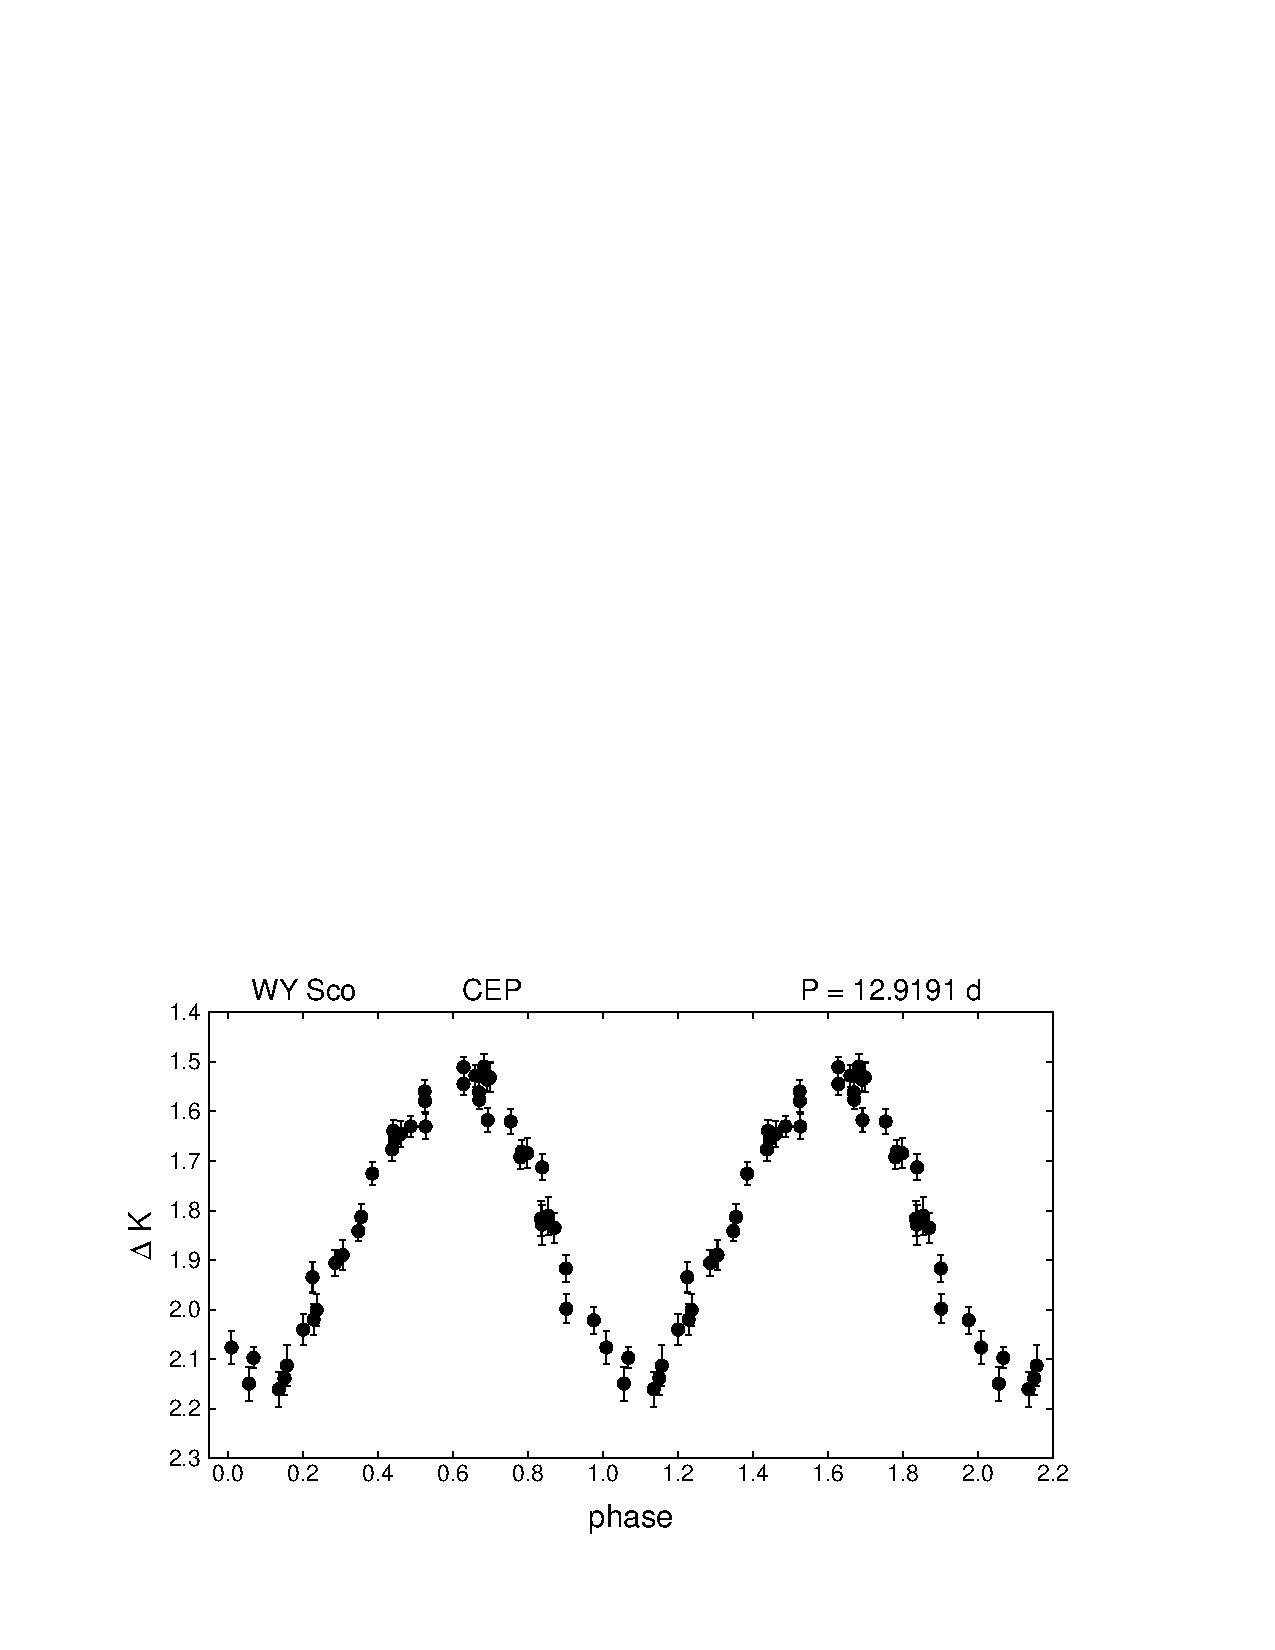
\includegraphics[width=0.8\textwidth]{04_antecedentes/figures/wys_opt.pdf}
    \caption{
       Observaciones de magnitud en la banda $K$ de la estrella \emph{Cepheid} WY Sco.
       El eje X representa la fase de medición. El eje Y, la magnitud en orden inverso.
       Crédito: \citet{catelan2011vvv}.
    }
    \label{fig:wys_opt}
\end{figure}


El gráfico de \autoref{fig:wys_opt} exhibe la \gls{lc} de una estrella \emph{Cepheid} puesta en fase. Los patrones regulares de aumento y disminución del brillo revelan el período de pulsación de la estrella. Además, la \gls{lc} expone detalles sobre la amplitud de los cambios de brillo, proporcionando información adicional sobre las propiedades físicas del objeto, como la masa y la composición química.
\section{El desafío de la era de los datos}

Con el advenimiento de nuevos telescopios y programas de observación, la astronomía ha ingresado en la era del \emph{Big Data}. Relevamientos masivos, como el \emph{Zwicky Transient Facility} \citep{bellm2018ztf}, tienen la capacidad de observar y monitorear millones de estrellas de manera continua y en múltiples bandas del espectro electromagnético, redefiniendo así los límites de la astronomía observacional y expandiendo nuestra comprensión del universo.

Uno de estos proyectos es el \acrfull{vvv} \citep{minniti2010vvv}, el cual hace uso del telescopio \gls{vista} ubicado en el Observatorio Paranal de Chile (\autoref{fig:vista}) para explorar el disco y el bulbo de la Vía Láctea en el infrarrojo cercano. Desde su inicio en 2010, el \gls{vvv} y su sucesor, el \gls{vvvx}, han llevado a cabo alrededor de 4200 horas de observación repartidas en un período de aproximadamente 13 años. En total, ha obtenido más de 350 mil imágenes, que componen un catálogo con más de $10^6$ archivos de observaciones \citep{saito2024vvvx}.

\begin{figure}[!ht]
    \centering
    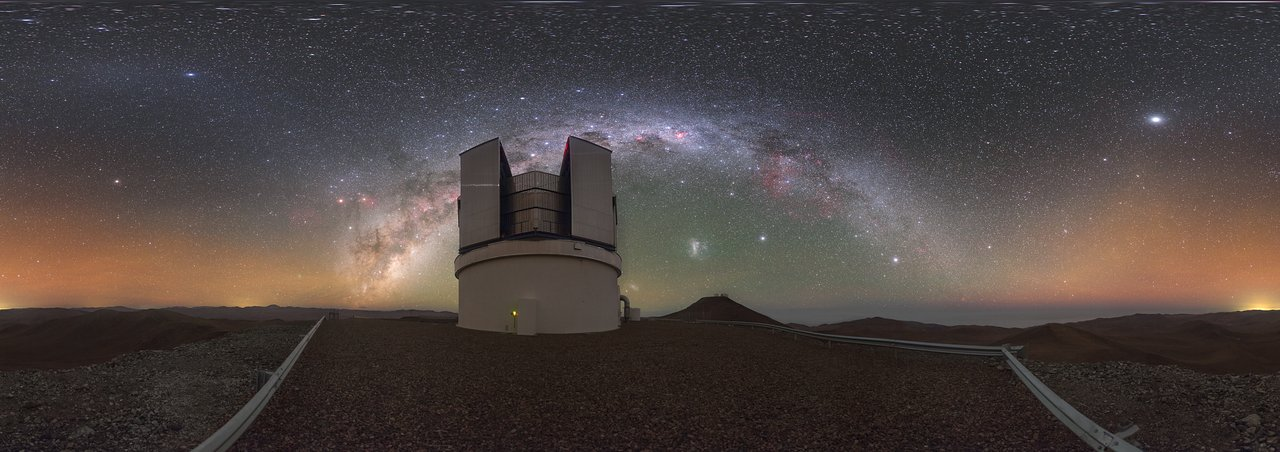
\includegraphics[width=0.8\textwidth]{04_antecedentes/figures/vista.jpg}
    \caption{
        El telescopio \acrfull{vista}, situado en el Observatorio Paranal de ESO, en Chile.
        Crédito: ESO/P. Horálek.
    }
    \label{fig:vista}
\end{figure}

Esta explosión de información no es exclusiva del \gls{vvv}. Proyectos similares como el futuro Observatorio Vera C. Rubin \citep{ivezi2019lsst} están preparados para producir volúmenes de datos aún mayores, presentando nuevos desafíos con respecto al manejo y análisis de estos datos en la astronomía moderna.

El creciente volumen y complejidad de los datos astronómicos hacen que el análisis manual de las observaciones sea inviable, volviendo indispensables el uso de nuevas técnicas automatizadas capaces de procesar información de manera eficiente. En este panorama, los algoritmos de \acrlongsp{ml} se han posicionado como herramientas clave para identificar patrones complejos que serían imposibles de detectar manualmente, abriendo nuevas puertas al conocimiento en una escala sin precedentes.


\section[Aprendizaje automático para la generación de conocimientos]{
    \Acrlongsp{ml} para la generación de conocimientos
}

El \acrfull{ml} es una rama de la inteligencia artificial que busca diseñar algoritmos capaces de aprender y mejorar a partir de datos, sin necesidad de reglas explícitas programadas. En términos simples, un programa se considera capaz de aprender si su desempeño en una tarea específica mejora con la experiencia \citep{mitchell1997machine}. Los algoritmos de \gls{ml} se pueden aplicar a grandes cantidades de datos para automatizar procesos complejos y mejorar la efectividad de tareas específicas, siendo las actividades de clasificación, regresión, optimización y agrupación las aplicaciones más comunes de los modelos de \gls{ml} \citep{michalski2013ml}.

El proceso por el cual se extrae conocimiento útil a partir de colecciones masivas de datos se denomina \gls{dm}. Esta técnica se apoya en gran medida en los algoritmos de \gls{ml} para identificar patrones y relaciones existentes entre los datos de manera automática y eficiente, lo que facilita el descubrimiento de información valiosa que de otro modo permanecería oculta.

Con el objetivo de sistematizar la generación de conocimiento a partir de volúmenes extensos de datos surge el método de \gls{kdd}. Inspirado en el método científico, \gls{kdd} define una serie de etapas secuenciales que buscan reducir la complejidad de los datos crudos para transformarlos en información útil y comprensible que puede ser utilizada para mejorar la toma de decisiones en diversos campos \citep{fayyad1996advances}. En la \autoref{fig:kdd} se aprecian las distintas etapas del proceso, que van desde la selección y el preprocesamiento de los datos hasta la interpretación y evaluación de los resultados.

\begin{figure}[!ht]
    \centering
    \makebox[\textwidth][c]{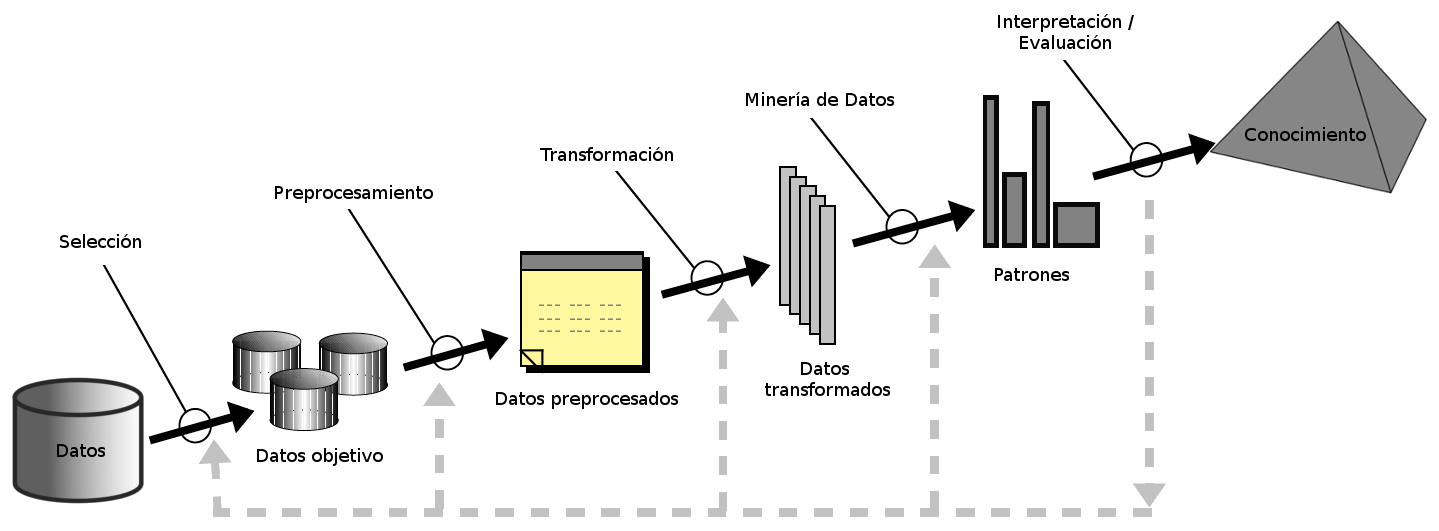
\includegraphics[width=1\linewidth]{04_antecedentes/figures/kdd.png}}
    \caption{
        Diagrama del procedimiento de KDD, adaptado de \citet{fayyad1996advances}.
    }
    \label{fig:kdd}
\end{figure}

El enfoque \gls{kdd} se sostiene principalmente en la fase de \gls{dm} como un puente entre los datos almacenados y el conocimiento. Si bien en la literatura es común utilizar los términos \gls{kdd} y \gls{dm} de manera intercambiable, en nuestro contexto hablaremos de \gls{dm} para referirnos específicamente a la etapa de identificación de patrones dentro del proceso completo de \gls{kdd}, el cual incluye las fases previas de preprocesamiento y transformación de los datos, así como la interpretación posterior de los resultados.

La efectividad de los algoritmos de \gls{ml} aplicados en la \acrlongsp{dm} está determinada por la calidad y representatividad de los datos que se utilicen como entrada. Las etapas de preprocesamiento y transformación son, entonces, fases especialmente importantes del enfoque \gls{kdd}, porque se encargan de limpiar y adaptar los datos crudos a una forma más fácil de manejar para los modelos de \gls{ml}. Este mecanismo no es automático; más bien, la naturaleza compleja de los datos hace que el proceso sea caro, tedioso y difícil, pues requiere de un conocimiento muy específico del dominio del problema para asegurar que los datos analizados son significativos.

En este trabajo nos enfocamos en la tarea de transformación de los datos para la reducción de complejidad y la identificación de atributos relevantes en los catálogos astronómicos. En particular, nos interesa la técnica de extracción de características, aplicada específicamente al estudio de \glspl{lc} para estrellas variables.

\section{Extracción de características}

Las \glspl{lc}, en su forma original como series temporales, constituyen datos de naturaleza inherentemente compleja y de alta dimensionalidad. Aunque contienen información valiosa sobre las propiedades físicas de las estrellas, esta se encuentra normalmente ofuscada por factores como la gran escala de los datos, el ruido instrumental y la incompletitud de las observaciones, haciendo del análisis de \glspl{lc} una tarea costosa incluso para los algoritmos avanzados de \gls{ml}.

Para abordar los problemas asociados a la complejidad de las \glspl{lc}, se emplea la técnica conocida como extracción de características \citep{khalid2014featureextraction}. Mediante este proceso, se transforman las series temporales originales en un conjunto de características clave que encapsulan la información más relevante para una representación más compacta y manejable de los datos.

Cuando hablamos de una característica, nos referimos a un descriptor cuantitativo que resume o representa algún aspecto importante del conjunto de datos. El conjunto completo de características define el llamado espacio de características, que conforma la representación final sobre la cual operan los modelos de \gls{ml}. Un espacio de características bien diseñado no solo reduce la carga computacional, sino que también mejora la capacidad del modelo para identificar patrones significativos, facilitando en nuestro caso tareas como la clasificación de estrellas variables y la predicción de parámetros físicos.

Las técnicas de extracción de características pueden involucrar tanto métodos manuales como automáticos. Los métodos automáticos se basan en técnicas de aprendizaje profundo como redes neuronales convolucionales \citep{chui2023convolutionalneuralnetwork} para derivar propiedades de manera implícita, partiendo únicamente de los datos; mientras que en los métodos manuales, en cambio, los investigadores definen explícitamente las características a calcular, seleccionando aquellas más relevantes en función del contexto.

Si bien los enfoques automáticos son útiles para identificar patrones en estructuras complejas, las características resultantes suelen ser limitadas en cuanto a su interpretabilidad, dificultando la comprensión física de los fenómenos. En contraste, el control que conceden los procesos manuales permite la extracción de propiedades con un significado físico claro, siendo este enfoque particularmente valioso en el panorama de \glspl{lc} al vincular las características extraídas con procesos observables. 

\section{Características de las curvas de luz}

En el análisis de \glspl{lc}, las características más efectivas son las que capturan las propiedades físicas de la estrella observada, como su periodicidad o su amplitud. Estas propiedades no solo son fácilmente interpretables, brindando información sobre los fenómenos subyacentes, sino que además simplifican la distinción entre los distintos tipos de estrellas variables. En el resto de esta sección, se detallan algunas de las características más relevantes de las \glspl{lc} empleadas en el análisis de estas estrellas.


\begin{description}
    \item[Período ($P$)]
    El período representa el tiempo que tarda una estrella variable en completar un ciclo completo de variación de brillo. Como ya dijimos, esta característica es especialmente conveniente en el caso de las \emph{Cepheid} y de las \emph{RR Lyrae}, porque posibilita el cálculo preciso de distancias astronómicas.
    
    El cálculo del período se realiza comúnmente mediante métodos espectrales como el de Lomb-Scargle \citep{lomb1976ls}, que identifica las frecuencias dominantes en los datos temporales. Siguiendo este método, el período se deriva como el inverso de la frecuencia principal:
    \[
    P = \frac{1}{f_{\max}}
    \]
    donde $f_{\max}$ es la frecuencia con mayor potencia en el espectro.

    \item[Amplitud ($A$)]
    Algunos tipos de estrellas pulsantes como las \emph{RR Lyrae} presentan amplitudes características en sus oscilaciones \citep{dallora2006rrlyraedistancescale}, por lo que se trata de una característica útil para clasificar las estrellas variables.
    
    La amplitud mide la diferencia entre el brillo máximo y mínimo registrado en la \gls{lc}. Por lo general, se suele considerar la mitad de esa diferencia con el fin de obtener una medida más representativa de la variación del brillo en torno al valor medio. La fórmula está dada por:
    
    \[
    A = \frac{\max{(m)} - \min{(m)}}{2}
    \]
    donde $m$ representa las magnitudes aparentes observadas.
    
    Cuando los datos contienen abundancia de ruido o de valores atípicos, se puede emplear un cálculo de la amplitud más robusto que considera las medianas del $5\%$ superior e inferior de las magnitudes observadas, en lugar de los máximos y mínimos absolutos \citep{richards2011timeseries}.
    
    \item[\emph{Skewness} ($G_1$)]
    El \emph{skewness} es una medida de la asimetría en la distribución de las magnitudes en una \gls{lc}. Matemáticamente, se define como:
    
    \[
    G_1 = \frac{N}{(N - 1)(N - 2)} \frac{\sum_i(m_i - \bar{m})^3}{\sigma_m^3},
    \]
    donde $N$ es el número de observaciones, $\bar{m}$ es la media muestral de la magnitud y $\sigma_m$ es la desviación estándar muestral \citep{joanes1998skewnesskurtosis}.
    
    Un valor positivo de asimetría indica una curva con un ascenso lento y un descenso rápido, mientras que un valor negativo indica lo opuesto. Esta característica es de utilidad para identificar la forma de las oscilaciones en estrellas pulsantes.
\end{description}

Además de las características ya mencionadas, existen otras propiedades estadísticas y dinámicas que enriquecen aún más el análisis de las \glspl{lc}. Algunas de estas, utilizadas por \citet{richards2011timeseries} en su trabajo para la clasificación de estrellas variables, son:
\begin{itemize}
    \item \emph{Frecuencia}: Relacionada con el período, indica la cantidad de ciclos por unidad de tiempo.
    \item \emph{Autocorrelación}: Evalúa la similitud entre diferentes puntos de la curva.
    \item \emph{Índice de variabilidad}: Mide la variabilidad global de la \gls{lc}, proporcionando una estimación cuantitativa de las fluctuaciones de brillo a lo largo del tiempo.
    \item \emph{Kurtosis}: Medición de la ``altitud'' y la ``anchura'' de los picos de la curva. Proporciona información sobre la concentración y la dispersión de los datos.
\end{itemize}

\section{Cómputo distribuido}

El volumen y complejidad de los datos astronómicos no sólo desafían nuestra capacidad de análisis, sino también las infraestructuras computacionales que los sustentan. A medida que la cantidad de datos a analizar sigue creciendo de manera exponencial, los sistemas tradicionales de procesamiento centralizado ya no son suficientes para enfrentar los desafíos de escalabilidad, eficiencia y rapidez que demandan las aplicaciones modernas. En este contexto, el cómputo distribuido proporciona una solución viable para paralelizar el preprocesamiento de datos \citep{zaharia2016stark}, el entrenamiento de modelos de \gls{ml} \citep{dean2012distributeddeepnetworks} y la ejecución de análisis en múltiples nodos \citep{abadi2016tensorflow}.

El concepto de cómputo distribuido se refiere a un paradigma de procesamiento en el que múltiples máquinas (o nodos) trabajan conjuntamente para resolver una tarea que no podría ser procesada de manera eficiente en un solo sistema \citep{tanenbaum2006distributedsystems, coulouris2011distributedsystems}. En este enfoque, los recursos de varios dispositivos, a menudo dispersos geográficamente y conectados por una red, se agrupan para ejecutar programas de manera colaborativa. Cada nodo en un sistema distribuido puede tener su propia memoria y CPU, y todos operan de forma coordinada, a menudo compartiendo información y procesando partes de un mismo problema en paralelo.

En términos de la estructura física de los sistemas, el concepto de cómputo distribuido no es una novedad, pues la idea de distribuir el trabajo entre varios equipos de computación se viene implementando desde hace varias décadas. Sin embargo, la reciente expansión del acceso a redes de alta velocidad y la mejora en la capacidad de los sistemas de comunicación han acelerado su adopción \citep{kurose2012networks}.

\section{Paralelismo y concurrencia}

Dentro de la construcción de sistemas de cómputo distribuidos, el paralelismo y la concurrencia representan bloques fundamentales para aprovechar al máximo los recursos disponibles del sistema \citep{silberschatz2012operatingsystems}. Mientras que el cómputo distribuido se encarga de coordinar múltiples nodos para abordar una tarea de gran escala, el paralelismo y la concurrencia se ocupan de explotar la capacidad interna de cada nodo, dividiendo el trabajo entre los múltiples núcleos de procesamiento que lo componen.

El paralelismo refiere a la ejecución simultánea de tareas. Esta técnica consiste en dividir un problema grande en varios subproblemas que puedan ser resueltos de forma independiente y en paralelo por diferentes unidades de cómputo. El objetivo es maximizar la utilización de los recursos disponibles, ya sean los núcleos de CPU o los nodos de una red distribuida, para acortar los tiempos de ejecución. Existen dos formas comunes de paralelismo:

\begin{itemize}
    \item \emph{Paralelismo de datos}. Se aplica la misma operación sobre diferentes conjuntos de datos en paralelo. Por ejemplo, entrenar un modelo de \gls{ml} sobre un \emph{data set} dividido \citep{dean2012distributeddeepnetworks}.
    
    \item \emph{Paralelismo de tareas}. Se ejecutan operaciones diferentes sobre un mismo conjunto de datos. Un caso típico
    es el procesamiento de imágenes, donde las operaciones disponibles son independientes entre sí \citep{saxena2016imageprocessing}.

\end{itemize}

Por otro lado, la concurrencia apunta a la gestión de múltiples tareas que progresan de forma simultánea, aunque no necesariamente se ejecuten exactamente al mismo tiempo. A menudo, la concurrencia se implementa para permitir que un programa realice operaciones mientras espera otras más lentas, como accesos a disco o llamadas de red, garantizando que ninguna tarea se quede estancada \citep{mccool2012parallel}.

En el ámbito de la programación, las ideas de paralelismo y concurrencia suelen implementarse mediante dos estrategias comunes:

\begin{description}
    \item[\emph{Multithreading}] (``multihilos'') 
    Se basa en el uso de múltiples hilos (\emph{threads}) de ejecución compartiendo un mismo espacio de memoria. Es una estrategia eficaz para programas que realizan muchas operaciones de entrada y salida, ya que permite que el sistema avance mientras espera la finalización de tareas bloqueantes.
    
    Los interpretes comunes de Python implementan un \gls{gil} que limita la ejecución concurrente de código Python puro, lo que restringe su efectividad en tareas intensivas de CPU \citep{piñeiro2024omp4pypurepythonimplementation}.

    \item[\emph{Multiprocessing}] (``multiprocesamiento'')
    Mediante esta técnica, se crean múltiples procesos aislados que no comparten memoria. A diferencia de los hilos, estos procesos sí pueden ejecutarse verdaderamente en paralelo, incluso sobre múltiples núcleos físicos, por lo que resulta especialmente útil cuando las tarea son independientes entre sí. En contraste, esta estrategia se ve comprometida cuando hay mucha comunicación entre procesos, pues presenta una mayor sobrecarga al no compartir una memoria.
 
    La separación de procesos permite que cada uno cuente con su propia instancia del intérprete de Python, sorteando así las limitaciones impuestas por el \gls{gil}.
\end{description}

La elección entre \emph{multithreading} y \emph{multiprocessing} depende de la naturaleza del problema, así como del entorno de ejecución. Como el \emph{multithreading} puede verse limitado por el \gls{gil}, suele emplearse cuando el problema involucra muchas operaciones de entrada y salida, mientras que las técnicas de \emph{multiprocessing} son más adecuadas cuando las tareas requieren alto poder de procesamiento y no necesitan compartir datos entre sí. En resumen: si el cuello de botella es la CPU, es preferible el \emph{multiprocessing}; si es la latencia de operaciones de I/O, \emph{multithreading} \citep{bienia2008parsec}. Entender estas distinciones resulta fundamental para desarrollar soluciones escalables y eficientes en contextos de análisis de datos de gran escala.


\section[Olores en el código: de FATS a feets]{
    Olores en el código: de \acrshort{fats} a \acrshort{feets}
}


\gls{fats} \citep{nun2015fatsfeatureanalysistime} es una herramienta diseñada para la extracción de características a partir de series temporales, particularmente de \glspl{lc} de objetos variables. Construida sobre el \emph{stack} científico de Python\footnote{\url{https://www.python.org/}}, \gls{fats} proporciona un \emph{framework} estandarizado que incluye extractores de características listos para usar, así como permite el desarrollo de nuevos extractores de manera flexible.

A pesar de las utilidades ofrecidas por \gls{fats}, su diseño e implementación han presentado diversas limitaciones que, a la larga, condujeron al desarrollo de su sucesor, \gls{feets}. Estas deficiencias se ven evidenciadas por la presencia de ``malos olores'' en el código, o \emph{code smells}.

Según \citet{fowler2006codesmell}, se les dice \emph{code smells} a
\begin{quote}
    ...indicios superficiales en el código que sugieren problemas más profundos en el sistema...
\end{quote}

En el caso de \gls{fats}, el análisis en profundidad de estos \emph{code smells} \citep{cabral2018fatsfeetsimprovementsastronomical} llevó a la identificación de varias problemáticas significativas como el uso de variables globales, la gestión inadecuada de errores y la implementación de código no estandarizado. Estos problemas, sumados a la falta de documentación y a la incompatibilidad con nuevas versiones de Python, impactaron negativamente en la usabilidad de la herramienta.

En respuesta a las limitaciones identificadas en \gls{fats} se llevó a cabo el desarrollo de una nueva herramienta, \acrfull{feets} \citep{cabral2018feets}. Este proyecto implicó una reingeniería completa de \gls{fats}, reestructurada para resolver los problemas clave detectados y agregar otras mejoras significativas, incluyendo avances como la eliminación de variables globales y la optimización de algoritmos para un mejor rendimiento. Además, \gls{feets} incluye una documentación detallada y posee una cobertura de pruebas del 90\%, garantizando un \emph{software} más robusto, accesible y confiable para la comunidad astronómica.

La transición de \gls{fats} a \gls{feets} se centró en mejorar el diseño y la arquitectura de la herramienta sin modificar sus funcionalidades principales, un proceso comúnmente conocido como refactorización de código. Este enfoque permite modificar el diseño interno del \emph{software} para mejorar su calidad, mientras se mantienen los resultados esperados para los usuarios finales.

\section{Refactorización y calidad de \emph{software}}

La refactorización de código, formalizada por \citet{fowler1999refactoring}, es un proceso en la ingeniería del \emph{software} orientado a mejorar la estructura interna del código sin alterar su comportamiento externo. El objetivo principal de la refactorización es mejorar la comprensión del código y su adaptación a futuros cambios.

Este proceso no se reduce a una sola técnica, sino que comprende un conjunto de varias prácticas que, en conjunto, mejoran el diseño del código. Por ejemplo, dividir funciones extensas en subfunciones más específicas aumenta la claridad del código y permite desarrollar pruebas más efectivas. Del mismo modo, adoptar nombres precisos para las variables, métodos y clases ayuda a mejorar su interpretación y mantenimiento \citep{martin2009clean}.

Más allá de la claridad y la organización del código, la refactorización impacta directamente en la calidad del \emph{software} \citep{kaur2017qualityrefactoring}. Un código bien estructurado no solo facilita su mantenimiento, sino que también influye en atributos clave que determinan su fiabilidad y sostenibilidad a largo plazo.

La calidad del \emph{software} se entiende como el grado en que un sistema, componente o proceso cumple con los requisitos especificados y las expectativas del usuario \citep{iso9126quality}. El concepto de calidad se asocia principalmente a la correcta funcionalidad del sistema y a su conformidad con los requerimientos, pero también abarca atributos no funcionales que son fundamentales para su sostenibilidad y evolución. Por ejemplo:
\begin{itemize}
    \item \emph{Mantenibilidad}: La capacidad de ser modificado fácilmente, ya sea para corregir defectos, mejorar su rendimiento o adaptarlo a nuevos requerimientos.

    \item \emph{Eficiencia}: El uso adecuado de los recursos del sistema, como el tiempo de procesamiento, la memoria y otros recursos computacionales.

    \item \emph{Usabilidad}: La facilidad con la que los usuarios pueden interactuar con el sistema.

    \item \emph{Escalabilidad}: La capacidad para manejar un aumento en la carga de trabajo o el volumen de usuarios sin degradar su rendimiento.
\end{itemize}
La refactorización, al mejorar la estructura y diseño interno del código, contribuye directamente a potenciar estos aspectos, esenciales para el desarrollo de \emph{software} robusto y adaptable.

\section{Principios para el diseño de \emph{software}}

El diseño de \emph{software} se refiere al proceso de definir la arquitectura y estructura de un sistema, así como la organización de sus componentes y las formas que interactúan entre sí. Un buen diseño debe buscar que el \emph{software} sea fácil de interpretar, mantener y extender a lo largo del tiempo.

Respaldadas por el principio básico ``divide y vencerás'', las estrategias comunes de diseño consisten en dividir un sistema complejo en componentes más pequeñas, fáciles de manipular. Aunque estas partes no son independientes, su separación facilita la cooperación entre sí dentro de una jerarquía organizada. Esta partición busca que cada componente pueda entenderse, implementarse y mantenerse de forma individual, lo que reduce la complejidad global del sistema como un todo \citep{martin2003agilesoftwaredevelopment}.

Para lograr la separación efectiva de responsabilidades, resulta esencial contar con una buena abstracción: una descripción del comportamiento externo de un componente que oculta sus detalles internos. La correcta implementación de estos aspectos da lugar a un diseño modular \citep{parnas1972modularization}, separado en unidades discretas que pueden ser diseñadas, implementadas, probadas y modificadas con facilidad, manteniendo un impacto mínimo (o nulo) sobre las demás partes del sistema. Para lograr una modularidad efectiva, el diseño debe considerar dos propiedades importantes: el acoplamiento y la cohesión de los módulos \citep{jalote1997integrated}.

\begin{description}
    \item[El acoplamiento] es un concepto intermodular que captura la noción de dependencia entre módulos. Dos módulos son independientes si cada uno puede funcionar completamente sin la presencia del otro. Cuanto mayor es la dependencia entre módulos, mayor es la complejidad de las interfaces, por lo que se desea reducir el acoplamiento lo más que se pueda. En lenguajes como Java\footnote{\url{https://docs.oracle.com/en/java/index.html}}, una alta cantidad de sentencias \texttt{import} puede ser un indicio de acoplamiento excesivo, ya que refleja una fuerte dependencia del módulo respecto de múltiples componentes externos.
    
    \item[La cohesión] caracteriza, en cambio, el vínculo intramodular, es decir la relación entre los elementos dentro de un módulo. Un módulo con alta cohesión realiza actividades muy relacionadas entre sí, mientras que uno con cohesión baja intenta abarcar varias responsabilidades distintas. Por lo general se busca que un módulo se encargue de una sola tarea específica, por lo que es deseable conservar una cohesión elevada. Un indicador de cohesión es la relación entre estado y comportamiento: si la mayoría de los métodos de un módulo accede a sus atributos privados, esto sugiere que el estado interno está bien integrado con su funcionalidad.
\end{description}

\subsection{SOLID para el diseño orientado a objetos}

En el diseño de \emph{software} no existe un conjunto rígido de pasos que garantice el éxito, pero sí existen principios fundamentados en la ingeniería del \emph{software} que guían el proceso de diseño hacia soluciones robustas, escalables y de alta calidad.

Los principios SOLID \citep{martin2000design}, por ejemplo, son un conjunto de cinco principios diseñados específicamente para la programación orientada a objetos. Constituyen una serie de prácticas que mejoran la estructura y la calidad del código para alinearlo a las propiedades de un buen diseño. Cada una de las siglas de SOLID representa un principio distinto:

\begin{enumerate}
    \item \emph{S -- Principio de Responsabilidad Única (SRP)}.
    Una clase debe tener una única razón para cambiar, es decir, debe ser responsable de una sola funcionalidad dentro del sistema.

    \item \emph{O -- Principio de Abierto-Cerrado (OCP)}.
    Los objetos o entidades debe estar abierto para su extensión pero cerrado para su modificación.

    \item \emph{L -- Principio de Sustitución de Liskov (LSP)}.
    Las clases derivadas deben poder sustituir a sus clases base sin alterar el comportamiento del sistema \citep{liskov1994subtyping}.

    \item \emph{I -- Principio de Segregación de Interfaces (ISP)}.
    Un cliente no debe implementar una interfaz que no utilice, ni debe depender de métodos que no use. Es preferible definir múltiples interfaces pequeñas y especializadas antes que una interfaz grande y genérica.
    
    \item \emph{D -- Principio de Inversión de Dependencias (DIP)}.
    Las módulos de alto nivel no deben depender de módulos de nivel más bajo, sino de abstracciones.
\end{enumerate}

\section{Algunos patrones de diseño}

A lo largo del tiempo, los desarrolladores han identificado soluciones recurrentes a problemas comunes en la arquitectura del \emph{software}, dando origen a los patrones de diseño. Estos patrones ofrecen soluciones estandarizadas para problemas específicos en la estructuración y comportamiento del sistema \citep{gamma1995designpatterns, shvets2018dive}. No son fragmentos de código listos para copiar y pegar, sino estructuras y principios que guían el diseño de soluciones eficaces. A continuación, exploraremos algunos de los patrones de diseño que fueron relevantes para la orquestación de este proyecto.

\subsection{Patrón \emph{Template Method}}

El patrón \emph{Template Method} define la estructura de un algoritmo complejo en una clase base y delega la implementación de pasos específicos a sus distintas subclases, permitiendo su personalización sin modificar la estructura general del algoritmo \citep{shvets2018dive}. Este enfoque permite reutilizar lógica común y adaptar su comportamiento en función de las necesidades de las distintas clases, garantizando la coherencia en la ejecución.

\begin{figure}[!ht]
    \centering
    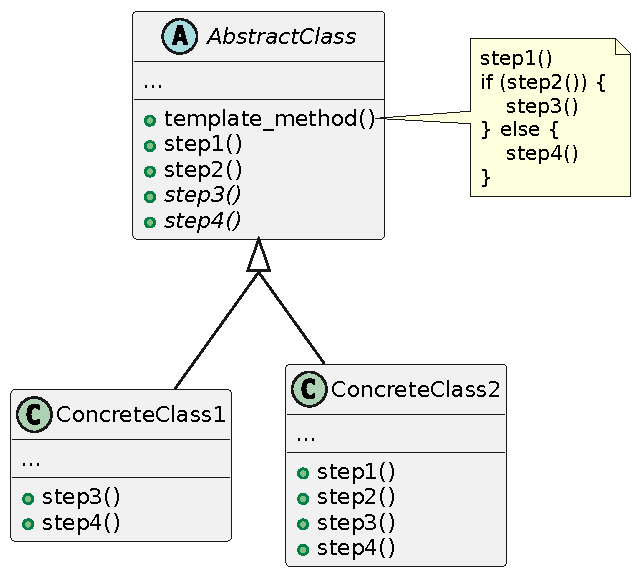
\includegraphics[width=0.55\textwidth]{04_antecedentes/figures/patterns/template_method.pdf}
    \caption{
        Diagrama UML que define el patrón \emph{Template Method}, extraído de \citet{shvets2018dive}. Los métodos abstractos se denotan por el uso de itálicas.
    }
    \label{fig:patterns/template_method}
\end{figure}

Como lo ilustra la \autoref{fig:patterns/template_method}, el patrón separa la estructura en dos tipos de clases:

\begin{description}
    \item[Una clase abstracta] (\texttt{AbstractClass}), que divide un algoritmo complejo en una serie de pasos, cada uno encapsulado en un método separado (\texttt{step1()}, \texttt{step2()}, \texttt{step3()} y \texttt{step4}()), y los integra ordenadamente dentro de un método de más alto nivel, el llamado ``\emph{template method}'' (\texttt{tem\-plate\_me\-thod()}).

  \item[Las subclases concretas] (\texttt{ConcreteClass1} y \texttt{ConcreteClass2}), que pueden reimplementar todos los pasos, pero sin alterar la lógica del \emph{template method}.
\end{description}

Algunos de los pasos individuales pueden ser abstractos, obligando a las subclases a proveer la implementación de su método correspondiente, mientras que los otros pueden ser opcionales, con una implementación predeterminada en la clase base, común para todas las subclases.

Para dar un ejemplo concreto, supongamos que queremos crear una aplicación destinada al análisis de documentos. Se espera que la aplicación funcione para distintos tipos de archivo (PDF, CSV y JSON), y que se pueda extender fácilmente a nuevos formatos si así se requiere. Después de analizar el problema, se redujo el proceso de análisis a cuatro etapas puntuales: \begin{enumerate}
    \item abrir el archivo que se desea analizar en modo de lectura
    \item extraer el texto del archivo
    \item procesar los datos extraídos
    \item generar un reporte con los resultados del análisis 
\end{enumerate}

\begin{figure}[!ht]
    \centering
    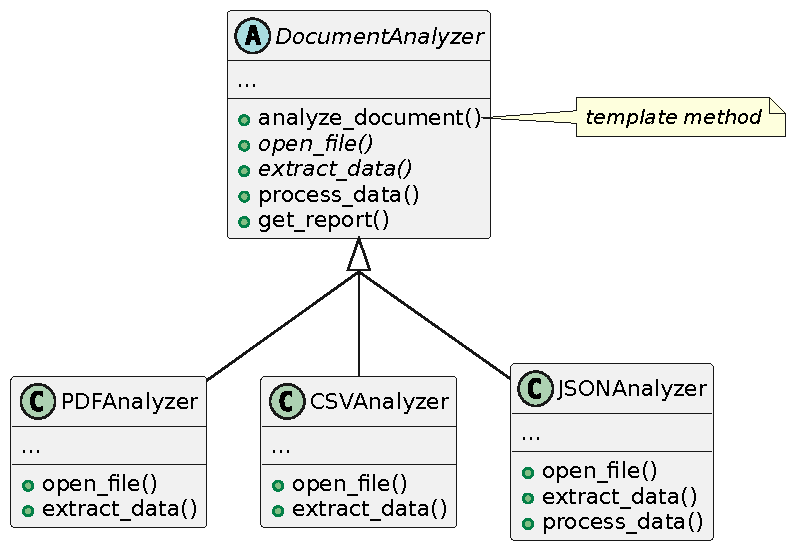
\includegraphics[width=0.725\textwidth]{04_antecedentes/figures/patterns/template_method_example.pdf}
    \caption{
        Diagrama UML del ejemplo del analizador de documentos, siguiendo el patrón \emph{Template Method}. Los métodos abstractos se denotan por el uso de itálicas.
    }
    \label{fig:patterns/template_method_example}
\end{figure}

Aplicando el patrón \emph{Template Method}, es posible llegar a un diseño como el de la \autoref{fig:patterns/template_method_example}.
La clase abstracta \texttt{DocumentAnalyzer} define el comportamiento del método \texttt{analyze\_document()} que funciona como un \emph{template method} para llevar a cabo el proceso completo de análisis. El algoritmo está separado en cuatro métodos diferentes, uno para cada paso identificado: \texttt{open\_file()}, \texttt{extract\_data()}, \texttt{process\_data()} y \texttt{get\_report()}.

Las subclases \texttt{PDFAnalyzer}, \texttt{CSVAnalyzer} y \texttt{JSONAnalyzer} implementan la lógica específica para el análisis de PDF, CSV y JSON respectivamente. Se determinó que los pasos de apertura de archivos y de extracción son muy dependientes del tipo de archivo analizado, por lo que sus métodos correspondientes se definen como abstractos, mientras que la lógica detrás del procesamiento y de la generación del reporte es muy similar para los distintos formatos de archivo, por lo que sus métodos constan de una implementación predefinida en la clase base.

\subsection{Patrón \emph{Facade}}

El patrón \emph{Facade} hace uso de una clase que proporciona una interfaz simplificada a un subsistema más complejo, actuando como una ``fachada''. De esta forma, reduce la dependencia de los clientes con las diferentes partes del subsistema.

Una fachada puede limitar las funcionalidades de los subsistemas a solo aquellas que requieran los clientes. Puede ser útil, por ejemplo, al querer integrar una aplicación con una biblioteca que provea decenas de funcionalidades, de las cuales solo se necesitan algunas pocas para solucionar el problema en cuestión.

\begin{figure}[!ht]
    \centering
    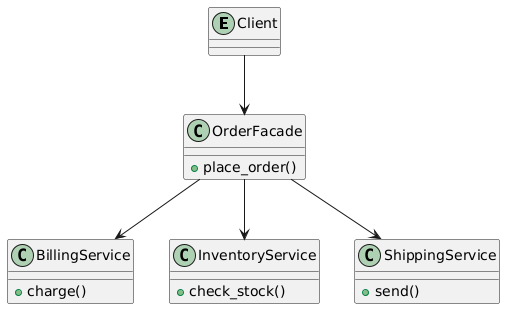
\includegraphics[width=0.75\textwidth]{04_antecedentes/figures/patterns/facade.png}
    \caption{
        Diagrama UML que define el patrón \emph{Facade}, extraído de \citet{shvets2018dive}.
    }
    \label{fig:patterns/facade}
\end{figure}

La \autoref{fig:patterns/facade} exhibe la estructura del patrón \emph{Facade}, que típicamente consiste de las siguientes partes:

\begin{description}
    \item[Una clase fachada] (\texttt{Facade}) que proporciona una interfaz conveniente para acceder a funcionalidades específicas del subsistema. Conoce cómo operar con las distintas partes del subsistema, y a dónde redirigir las solicitudes del cliente.

    \item[Otras fachadas] (\texttt{AdditionalFacade}) que pueden ser opcionalmente creadas para evitar tener una sola fachada con varias funcionalidades no relacionadas, reduciendo su complejidad. Estas fachadas adicionales pueden ser utilizadas tanto por el cliente como por las otras fachadas.

    \item[El subsistema complejo] (\texttt{ComplexSubsystem}) con múltiples componentes que proveen distintas funcionalidades. Normalmente, uno tendría que involucrarse con los detalles de implementación del subsistema para poder utilizar sus funcionalidades de la forma correcta. Las clases del subsistema (\texttt{SubsystemClass1}, \texttt{SubsystemClass2}, etc.) no deberían ser conscientes de la existencia de la fachada, sino que se comunican directamente entre sí sin operar por fuera del subsistema.

    \item[El cliente] que hace uso de la fachada sin hacer llamadas directas al subsistema.
\end{description}

Pongamos como ejemplo una aplicación de gestión de pedidos, que cuenta con servicios internos que se ocupan de distintas tareas: facturación, inventario y envío. La \autoref{fig:patterns/facade_example} visualiza el uso del patrón \emph{Facade} para tal ejemplo, donde la aplicación se comunica directamente con la clase \texttt{OrderFachade} que actúa como una fachada para ordenar la comunicación con las funcionalidades respectivas de los distintos servicios (\texttt{BillingService}, \texttt{InventoryService} y \texttt{ShippingService}).

\begin{figure}[!ht]
    \centering
    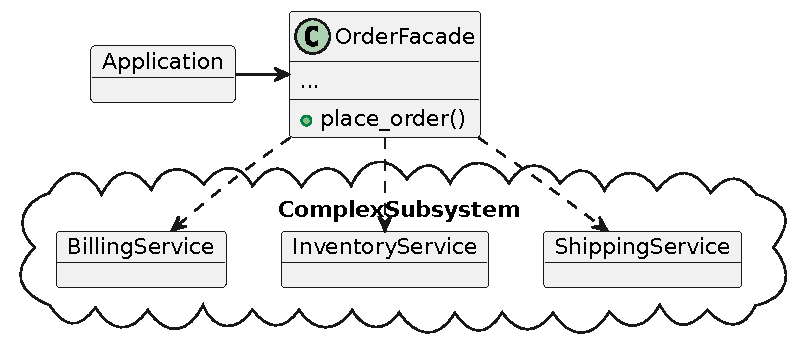
\includegraphics[width=0.75\textwidth]{04_antecedentes/figures/patterns/facade_example.pdf}
    \caption{
        Diagrama UML del ejemplo del gestor de pedidos siguiendo el patrón \emph{Facade}.
    }
    \label{fig:patterns/facade_example}
\end{figure}

\section{Métricas de calidad}

Empleando análisis estático sobre el código fuente de un sistema, es posible obtener ciertas métricas cuantitativas para estimar una noción objetiva de su calidad. La aplicación sistemática de estas métricas permite priorizar las áreas más problemáticas y enfocar los esfuerzos de refactorización donde se necesiten con mayor urgencia \citep{chidamber1994metrics, fowler1999refactoring}. A continuación, se describen las métricas más relevantes para los fines de este trabajo.

\subsection[Complejidad ciclomática (CC, Cyclomatic Complexity)]{
    \Gls{cc}
}

La \acrlongsp{cc}, propuesta por \citet{mccabe1976complexity}, mide la cantidad de caminos linealmente independientes en el flujo de control de un programa. Se suele usar este valor como una representación de la dificultad para entender, probar y mantener el código.

Se calcula a partir del grafo de flujo de control del programa con la siguiente fórmula:
\[
\text{CC} = E - N + 2P
\]
en donde:

\begin{align*}
    E&: \text{Número de aristas (conexiones entre nodos),} \\
    N&: \text{Número de nodos (bloques de código), y} \\
    P&: \text{Número de componentes conectados (p. ej.: funciones o métodos).}
\end{align*}

Un valor alto de \gls{cc} indica que el código tiene demasiadas bifurcaciones, lo que dificulta su mantenimiento. Idealmente, debería tener un valor menor a 10 para cada función o método.

\subsection{Métricas de Halstead}

Las métricas de Halstead \citep{halstead1977metrics} evalúan propiedades cuantitativas del código relacionadas con su tamaño, su complejidad y el esfuerzo necesario para desarrollarlo.

A partir del código fuente, se pueden obtener los siguientes valores: \begin{align*}
    N_1&: \text{Número total de operadores,} \\  
    N_2&: \text{Número total de operandos,} \\ 
    \eta_1&: \text{Número de operadores únicos,} \\
    \eta_2&: \text{Número de operandos únicos.}
\end{align*}
Estos números dan lugar al cálculo de varias métricas distintas. A continuación, algunas de ellas: \begin{align*}
    \text{Longitud del programa (N)}&: N = N_1 + N_2 \\
    \text{Volumen (\acrshort{hv})}&: V = N \log_2\eta \\
    \text{Esfuerzo (E)}&:E = V \frac{\eta_1}{2 \eta_2}
\end{align*}

\subsection[Líneas de código (LOC, Lines Of Code)]{
   \Gls{loc}
}

Es una métrica para evaluar el tamaño del \emph{software}. Tal como lo indica su nombre, es el número total de líneas en el código fuente. Aunque es fácil de calcular, debe usarse en combinación con otras métricas para evitar conclusiones simplistas. Se puede clasificar en:

\begin{itemize}
    \item \emph{Líneas de código físicas}: Todas las líneas en el archivo, incluidas las vacías y comentarios.  
    \item \emph{Líneas de código funcionales}: Solo las líneas con lógica ejecutable.
\end{itemize}

\subsection[Índice de mantenibilidad (MI, Maintainability Index)]{
   \Acrfull{mi}
}

El \acrlongsp{mi} determina qué tan fácil de mantener es el código: cuanto más alto sea el valor de la métrica, más fácil es el código de mantener. El cálculo, propuesto originalmente por \citet{oman1992metrics}, involucra varias de las métricas de calidad ya mencionadas: \gls{loc}, \gls{cc} y el \acrfull{hv}. Su valor está dado por la siguiente fórmula:
\[
\text{MI} = 171 - 5.2 \ln{V} - 0.23 \text{CC} - 16.2 \ln{\text{LOC}}
\]

La métrica fue más adelante refinada por \citet{coleman1994maintainability} y promovida por el \gls{sei} \citep{bray1997c4} incorporando además el \gls{poc}, el porcentaje de líneas de código del programa que conforman los comentarios:
\[
\text{MI}_\text{SEI} = 171 - 5.2 \ln{V} - 0.23 \text{CC} - 16.2 \ln{\text{LOC} + 50 \sin{\sqrt{2.46 \text{POC}}} }
\]

Otra variante de esta métrica, adoptada por Microsoft para el entorno de desarrollo de Visual Studio \citep{microsoft2025mi}, ajusta la fórmula a una escala fija entre el 0 y el 100:

\[
\text{MI}_\text{VS} = \max \{ 0, \frac{100}{171} (171 - 5.2 \ln{V} - 0.23 \text{CC} - 16.2 \ln{\text{LOC}}) \}
\]

En esta última variante, un valor mayor o igual a 20 indica un código fácil de mantener, y valores por debajo de 10 sugieren problemas significativos de mantenimiento.
 \cleardoublepage
\chapter[feATURE eXTRACTOR FOR tIME sERIES]{
    \acrlong{feets}
}
\label{chapter:feets}

\acrfull{feets} \citep{cabral2018feets} es una biblioteca de Python diseñada para la extracción de características en series temporales, haciendo énfasis en el estudio de \acrfullpl{lc}. Entre sus funcionalidades, incluye herramientas para el modelado, clasificación, limpieza de datos, detección de valores atípicos y análisis de catálogos fotométricos.

La herramienta proporciona un \emph{framework} especializado para la creación de extractores de características. Cuenta, también, con un conjunto estandarizado de \emph{features} listos para usar, que abarcan desde medidas estadísticas básicas como la media o la desviación estándar, hasta características complejas y específicas de las \glspl{lc} \citep{gran2015bulge}, como la función de autocorrelación. A pesar de su enfoque en el análisis de \glspl{lc}, \gls{feets} no se limita solamente al campo astronómico, sino que puede aplicarse a otras series temporales.

El proyecto surge como una refactorización integral de \gls{fats} \citep{nun2015fatsfeatureanalysistime}, con el objetivo de corregir deficiencias en su diseño, optimización y compatibilidad con versiones modernas de Python \citep{cabral2018fatsfeetsimprovementsastronomical}. Gracias a su arquitectura modular y mejorada, \gls{feets} facilita el procesamiento de grandes volúmenes de datos astronómicos e integra bibliotecas como \emph{AstroPy}\footnote{\url{https://www.astropy.org/}} para mejorar su interoperabilidad dentro del ecosistema de herramientas de astroinformática.

\section{Uso de la herramienta}

En este trabajo nos centraremos en el uso de \gls{feets} sobre el dominio de las \acrlongplsp{lc} astronómicas. No obstante, es importante destacar que la herramienta no se restringe únicamente al campo astronómico, sino que puede aplicarse sobre cualquier serie temporal que cuente con los vectores de datos necesarios.

En pocas palabras, \gls{feets} recibe como entrada los vectores de datos que componen una serie y devuelve un arreglo con las características computadas. El conjunto de características disponibles depende de los datos proporcionados por el usuario: si solo cuenta con vectores de magnitud y de tiempo, entonces solo se calcularán las características que puedan extraerse a partir de estos valores.

Para calcular el conjunto completo de características a partir de una \gls{lc}, la herramienta necesita de los siguientes vectores de datos:
\begin{itemize}
    \item \texttt{magnitude}. Magnitudes observadas.
    \item \texttt{time}. Tiempos de observación de \texttt{magnitude}.
    \item \texttt{error}. Errores asociados a \texttt{magnitude}.
    \item \texttt{magnitude2}. Magnitudes observadas en una banda diferente.
    \item \texttt{aligned\_magnitude}. Valores de \texttt{magnitude} temporalmente sincronizados con los de \texttt{magnitude2}.
    \item \texttt{aligned\_magnitude2}. Valores de \texttt{magnitude2} temporalmente sincronizados con los de \texttt{magnitude}.
    \item \texttt{aligned\_time}. Tiempos de observación compartidos entre \texttt{a\-ligned\_mag\-ni\-tude} y \texttt{aligned\_magnitude2}.
    \item \texttt{aligned\_error}. Errores asociados a \texttt{aligned\_magnitude}.
    \item \texttt{aligned\_error2}. Errores asociados a \texttt{aligned\_magnitude2}.
\end{itemize}
De estos, los vectores de magnitud y de tiempo son estrictamente necesarios para la ejecución porque son requeridos para el cálculo de todas las características disponibles. Los demás vectores son opcionales, requeridos solamente por algunas características específicas.

El \autoref{code:usage} ilustra el funcionamiento básico de \gls{feets} para la extracción de características de una \gls{lc} simulada. A continuación se describe paso a paso lo que hace el código:

\begin{enumerate}
    \item En las líneas 1 y 2, se importan las dependencias necesarias: \texttt{feets}, para hacer uso de la herramienta de extracción de características, y \texttt{numpy}, para la generación de datos numéricos simulados.

    \item En las líneas 4 y 5, se generan los vectores que conforman la \gls{lc}: se simulan aleatoriamente 30 valores para la magnitud aparente, y se generan sus 30 tiempos de observación asociados. En la línea 6, ambos vectores se agrupan en una lista que representa la \gls{lc} simulada.

    \item En la línea 8, se crea un espacio de características (\texttt{FeatureSpace}) indicando que se proporcionarán únicamente los vectores de magnitud y tiempo. Esta configuración determina qué subconjunto de características será calculado.

    \item En la línea 9, se llama al método \texttt{extract()} para extraer automáticamente las características de la \gls{lc} simulada. Este método devuelve dos listas: una con los nombres de las características extraídas y otra con sus valores correspondientes.

    \item Finalmente, en la línea 11, se reorganizan las características y sus valores en el diccionario \texttt{fdict}, mejorando su representación para un procesamiento posterior.
\end{enumerate}

\begin{code}
\begin{minted}{pycon}
>>> import feets
>>> import numpy as np

>>> time = np.arange(30)
>>> magnitude = np.random.rand(30)
>>> lc = [time, magnitude]

>>> fs = feets.FeatureSpace(data=["time", "magnitude"])
>>> features, values = fs.extract(*lc)

>>> dict(zip(features, values))
{'Amplitude': 0.4400277612857634,
 'AndersonDarling': 0.8117749648312879,
 'Autocor_length': 1.0,
 'Con': 0.0,
 'Eta_e': 2.0654257245579264,
 ...
 'PeriodLS': 0.052641132691958616,
 'Period_fit': 1.0,
 'Psi_CS': 0.1892202321018822,
 'Psi_eta': 1.5441584299683062,
 'Q31': 0.3968494550357215,
 'Rcs': 0.21378454173755806,
 'Skew': 0.25929379112189904,
 'SlottedA_length': 1.0,
 'SmallKurtosis': -0.6405350057567984,
 'Std': 0.2597002131031463,
 'StructureFunction_index_21': 1.8028982695940259,
 'StructureFunction_index_31': 2.4687064391908753,
 'StructureFunction_index_32': 1.40457469223505}
\end{minted}
\caption{
    Ejemplo del uso de \gls{feets} para la extracción de características de una \gls{lc} simulada con magnitudes aleatorias.
}
\label{code:usage}
\end{code}


\section{Funcionalidades}

Además de todo lo mencionado, \gls{feets} ofrece las siguientes funcionalidades:

\begin{description}
    \item[Extracción de características]
     La biblioteca cuenta con varios extractores listos para usar, los cuales permiten calcular más 40 características a partir de una \gls{lc}. Estas características incluyen medidas estadísticas, indicadores de periodicidad y métricas específicas de variabilidad.
     
     La lista completa de las características presentes en \gls{feets} se puede visualizar en la \autoref{table:features}.

    \item[Base para la creación de extractores]
    Además de los extractores preinstalados en la biblioteca, \gls{feets} incorpora un \emph{framework} para crear extractores de características propios.
    
    Cada extractor constituye una clase de Python. Esta clase debe extender la metaclase \texttt{feets.Extractor} con atributos que definan los datos de la serie temporal requeridos por el extractor (\texttt{data}) y las características que puede computar (\texttt{features}). También debe implementar el método \texttt{fit()}, que contiene la lógica de extracción de características.

    El \autoref{code:extractor} es un ejemplo de un extractor simple que computa el número de observaciones en una serie temporal. Toma como entrada los tiempos de observación de la muestra y devuelve un diccionario con la característica \texttt{Count}.

    El cálculo de las características de un extractor puede depender de los resultados obtenidos por otro. Estas dependencias deber ser especificadas en el atributo \texttt{dependencies} de la clase. Adicionalmente, un extractor puede contar con parámetros opcionales, personalizables por el usuario. Cada parámetro debe contar con un valor predeterminado el cual es asignado por el extractor en caso de no ser evaluado manualmente por el usuario. Los parámetros disponibles y sus valores predeterminados se deben declarar bajo el atributo \texttt{params}.
\end{description}

\begin{table}[!ht]
    \centering
    \begin{tabular}{||p{4cm}|p{7cm}||}
        \hline

         Datos de entrada
         &
         Características
         \\

        \hline
        \hline

        \texttt{magnitude}
        & 
        \texttt{Amplitude},
        \texttt{AndersonDarling},
        \texttt{Autocor\_length},
        \texttt{Con},
        \texttt{FluxPercentileRatioMid20},
        \texttt{FluxPercentileRatioMid35},
        \texttt{FluxPercentileRatioMid50},
        \texttt{FluxPercentileRatioMid65},
        \texttt{FluxPercentileRatioMid80},
        \texttt{Gskew},
        \texttt{Mean},
        \texttt{Meanvariance},
        \texttt{MedianAbsDev},
        \texttt{MedianBRP},
        \texttt{PairSlopeTrend},
        \texttt{PercentAmplitude},
        \texttt{PercentDifferenceFluxPercentile},
        \texttt{Q31},
        \texttt{Rcs},
        \texttt{Skew},
        \texttt{SmallKurtosis},
        \texttt{Std}.
        \\

        \hline

        \texttt{magnitude}, 
        \texttt{time}
        &
        \texttt{Eta\_e},
        \texttt{Freq{i}\_harmonics\_amplitude\_{j}},
        \texttt{LinearTrend},
        \texttt{MaxSlope},
        \texttt{PeriodLS},
        \texttt{Period\_fit},
        \texttt{Psi\_CS},
        \texttt{Psi\_eta},
        \texttt{SlottedA\_length},
        \texttt{StructureFunction\_index\_21},
        \texttt{StructureFunction\_index\_31},
        \texttt{StructureFunction\_index\_32}.
        \\
        
        \hline
        
        \texttt{magnitude}, 
        \texttt{error}
        &
        \texttt{Beyond1Std},
        \texttt{StetsonK}.
        \\
        
        \hline
        
        \texttt{magnitude}, 
        \texttt{time},
        \texttt{error}
        &
        \texttt{CAR\_mean},
        \texttt{CAR\_sigma},
        \texttt{CAR\_tau},
        \texttt{StetsonK\_A}.
        \\
        
        \hline
        
        \texttt{magnitude}, 
        \texttt{magnitude2}
        &
        \texttt{Color}.
        \\
        
        \hline
        
        \texttt{aligned\_magnitude}, 
        \texttt{aligned\_magnitude2}
        &
        \texttt{Q31\_color}.
        \\
        
        \hline
        
        \texttt{aligned\_magnitude}, 
        \texttt{aligned\_magnitude2},
        \texttt{aligned\_time}
        &
        \texttt{Eta\_color}.
        \\
        
        \hline
        
        \texttt{aligned\_magnitude}, 
        \texttt{aligned\_magnitude2},
        \texttt{aligned\_error},
        \texttt{aligned\_error2},
        &
        \texttt{StetsonJ},
        \texttt{StetsonL},
        \\
        
        \hline
    \end{tabular}
    \caption{
        Características presentes en \gls{feets} según sus datos de entrada.
    }
    \label{table:features}
\end{table}

\begin{code}
\begin{minted}{python}
from feets import Extractor

class Count(Extractor):
    # datos requeridos por el extractor para calcular las características
    data = ["time"]
    
    # características computadas por el extractor
    features = ["Count"]

    def fit(self, time):
        # el extractor computa la cantidad de observaciones a partir de los tiempos registrados
        count = len(time)

        # finalmente, devuelve un diccionario con las caracteríticas calculadas
        return {"Count": count}
\end{minted}
\caption{
    Extractor que computa la cantidad de observaciones en una serie temporal.
}
\label{code:extractor}
\end{code}

\begin{description}[resume]
    \item[Selección flexible de características]
    La herramienta provee una \gls{api} para la selección de varias características antes de su extracción. La clase \texttt{feets.FeatureSpace}, por defecto, calcula todas las características disponibles a la vez, pero puede ser instanciada con distintos parámetros de selección para determinar las características a computar.

    Como se mencionó anteriormente, las características se dividen según los vectores de datos necesarios para su extracción (\texttt{magnitude}, \texttt{time}, \texttt{error}, \texttt{magnitude2}, entre otros). Si el usuario no cuenta con todos estos datos, puede especificar el parámetro \texttt{data} con los vectores disponibles. Luego, la herramienta se encarga de seleccionar solo las características válidas bajo ese dominio de entradas. En caso de no especificar ningún dato, se seleccionan automáticamente todas las características.

    En lugar de extraer todas las características disponibles, el usuario puede decidir pasar el parámetro \texttt{only} con una lista de las características específicas que desea calcular. Similarmente, también puede excluir características de la selección mediante el parámetro \texttt{exclude}.

    \item[Limpieza y preprocesamiento de datos]
    Se incluyen dos utilidades para el preprocesamiento de datos de \glspl{lc}.
    La primera es la función \texttt{remove\_noise()} del módulo \texttt{feets.preprocess} que elimina los puntos de ``ruido'' en una \gls{lc}, es decir, aquellos que se encuentren a cinco desviaciones estándar de la media.
    La otra función del mismo módulo, \texttt{align()}, sincroniza dos \glspl{lc} en bandas observacionales distintas y obtiene los datos alineados (\texttt{aligned\_time}, \texttt{aligned\_magnitude}, \texttt{aligned\_magnitude2}, \texttt{a\-ligned\_e\-rror} y \texttt{a\-ligned\_e\-rror2}).

    
    \item[Lector de catálogos astronómicos]
    La biblioteca se integra con los relevamientos astronómicos \gls{ogle} \citep{soszynski2013ogle} y \gls{macho} \citep{alcock2001macho}. Incorpora funciones para descargar e interpretar los datos de los catálogos provenientes de estos proyectos. 

    \item[Generación de curvas de luz]
    Se incluye la capacidad de generar \glspl{lc} aleatorias. Hace posible la creación de \glspl{lc} con datos que sigan, por ejemplo, una distribución normal o uniforme. También permite generar \glspl{lc} con patrones de periodicidad específicos.

    \item[Documentación extensa]
    La documentación de \gls{feets} es completa y detallada. Incluye descripciones para los distintos módulos, clases y métodos del sistema, ayudando al entendimiento del código fuente de la biblioteca.
    También cuenta con un tutorial que resume la herramienta y explica sus distintas funcionalidades, con ejemplos prácticos y fáciles de entender.
\end{description}

\section{Arquitectura}

La estructura de \gls{feets} está dividida en cuatro módulos principales:

\begin{description}
    \item[\texttt{feets.core}] Provee la \gls{api} principal del sistema, el \texttt{FeatureSpace}. Mediante esta clase, el usuario puede elegir las características a computar o seleccionarlas a partir de los vectores de datos disponibles.

    En base a las características seleccionadas, el \texttt{FeatureSpace} se encarga de inicializar, parametrizar y orquestar la ejecución de los extractores en el orden necesario, asegurándose de que se cumplan las dependencias establecidas entre los distintos extractores.

    \item[\texttt{feets.extractors}] Módulo que implementa la lógica de los extractores de características y las herramientas para crear extractores propios. Contiene a la clase \texttt{Extractor}, que constituye la base de todos los extractores.
    
    El módulo cuenta también con un registro de todos los extractores y características disponibles en el sistema. El registro se asegura de que cada característica es extraída por su propia clase, y que cada extractor puede computar al menos una característica.
    
    El proceso para crear un nuevo extractor de características involucra crear una clase que herede de \texttt{Extractor}. Esta clase, además de implementar la lógica de extracción, debe incluir atributos que definan tanto las características generadas como los vectores de datos requeridos para la computación. Para hacer visible esta nueva clase al resto de la librería hay que agregarla al registro mediante la función \texttt{register\_extractor()}.

    \item[\texttt{feets.preprocess}] Proporciona funciones de limpieza y de preprocesamiento para los datos de series temporales. Las funciones \texttt{remove\_noise()} y \texttt{align()} mencionadas anteriormente pertenecen a este módulo.

    \item[\texttt{feets.datasets}] Provee una interfaz con funcionalidades básicas para la recuperación de catálogos. En particular, incluye implementaciones para la integración con los relevamientos astronómicos \gls{macho} y \gls{ogle}, pero puede extenderse a otros proyectos. Este módulo también incorpora funciones para la generación de \glspl{lc} con datos aleatorios.
\end{description}

Es importante resaltar la división entre la funcionalidad de análisis y la de creación de extractores de características. Esta separación simplifica la operación del sistema y posibilita la implementación de extractores complejos.

\section{Limitaciones}

A pesar de sus funcionalidades, identificamos algunas limitaciones en la implementación actual de \gls{feets} que pueden afectar su uso en algunos escenarios:

\begin{description}
 \item[Ejecución secuencial de los extractores]
    El algoritmo de extracción modelado por \gls{feets} sigue un modelo de planificación secuencial. Esto significa que, dada una selección de extractores, el programa empieza por ejecutar alguno de ellos y, una vez completada la ejecución, procede con el cálculo del siguiente. Luego de finalizar el segundo extractor se pasa al tercero; y así sucesivamente hasta haber pasado por todos los extractores.
    
    Si bien este algoritmo cumple con su cometido, es fácil notar que el tiempo de ejecución de todo el procedimiento aumenta linealmente con la cantidad de extractores utilizados. Esto supone un cuello de botella significativo cuando se trabaja con varios extractores a la vez, lo que puede volverse una limitación importante en contextos donde se analizan miles de \glspl{lc}.
    
    Si bien los extractores de \gls{feets} pueden presentar dependencias entre sí, en la práctica la mayoría de estos son capaces de operar de manera completamente autónoma. El modelo secuencial, entonces, podría reemplazarse por un algoritmo más inteligente que realice una ejecución en simultáneo de los extractores, de lo posible. Tal enfoque no solo aprovecharía mejor los recursos del sistema, si no que puede reducir significativamente los tiempos de ejecución al trabajar con grandes volúmenes de datos.

    \item[Configuración limitada del \texttt{FeatureSpace}] 
    La interfaz de \texttt{FeatureSpace} no comprende el procesamiento de varias \glspl{lc} en simultáneo dentro de una misma ejecución. Esto presenta una desventaja en análisis que requieran la comparación en tiempo real de diferentes fuentes de datos, en donde se trabaja con múltiples \glspl{lc} de las cuales se buscan extraer las mismas características.

    Sumado a esto, en el mismo \texttt{FeatureSpace} no es posible instanciar un extractor con diferentes parámetros. Esto significa que si un usuario desea calcular una métrica con distintas configuraciones, debe crear múltiples instancias de \texttt{FeatureSpace} separadas, o que puede resultar en una mayor carga computacional y en una estructura de código más compleja de mantener. Esta limitación impide realizar experimentos de sensibilidad sobre los parámetros de los extractores de manera eficiente.

    \item[Uso de metaclases en lugar de clases abstractas]
    En Python, todo es un objeto, incluyendo las mismas clases: así como un objeto es una instancia de una clase, una clase es una instancia de lo que se conoce como una metaclase \citep{python2025python}. Las metaclases permiten modificar el comportamiento de las clases en el momento de su creación, sin embargo, un gran poder conlleva una gran responsabilidad. Las metaclases pueden generar comportamientos inesperados en sus instancias, dificultando el \emph{debugging} y \emph{testing}. Sumado a esto, la utilización de metaclases suele seguirse del uso de técnicas avanzadas de metaprogramación que reducen la legibilidad del código y complican aún más su mantenimiento.

    En el caso de \gls{feets}, la creación de las clases de extractores se hace a partir de la metaclase \texttt{Extractor}, la cual valida que se implemente el método de extracción necesario y que las definiciones de los atributos sean correctas. Estas restricciones establecen un contrato común, que le permite a la herramienta y al usuario poder hacer suposiciones sobre el comportamiento de los extractores.

    El contrato establecido por la metaclase \texttt{Extractor} puede implementarse de una manera más simple reemplazando el uso de una metaclase por el de una clase abstracta. Esto es, una clase especial que no puede ser instanciada directamente, sino que establece una interfaz común para sus subclases. En Python, las clases abstractas se implementan utilizando el módulo \texttt{abc}, que permite declarar métodos abstractos sin necesidad de recurrir a la metaprogramación. Este enfoque simplificaría el código y mejoraría su legibilidad, evitando la complejidad adicional de las metaclases y haciendo que las reglas de validación sean más explícitas.

    \item[Persistencia de las configuraciones]
    Una funcionalidad faltante de \gls{feets} es la de un mecanismo para guardar y reutilizar la configuración de un \texttt{Fea\-ture\-Space}. Esto significa que los usuarios deben reconfigurar manualmente sus selecciones de características cada vez que ejecutan el programa, lo que puede ser poco práctico en flujos de trabajo repetitivos. 
    
    En escenarios donde se requiere ejecutar análisis con configuraciones predefinidas, la ausencia de una funcionalidad de persistencia obliga a los usuarios a implementar soluciones externas, como la escritura manual de archivos de configuración o el uso de bases de datos. La inclusión de una funcionalidad que permita la serialización y deserialización de configuraciones de \texttt{FeatureSpace} mejoraría significativamente la usabilidad de la heramienta y permitiría una integración más sencilla con otros sistemas de procesamiento de datos.

    \item[Mantenimiento de versiones obsoletas]
    Si bien \gls{feets} es compatible con la versión 3 de Python, aún mantiene soporte para Python 2, versión oficialmente descontinuada desde enero de 2020\footnote{\url{https://devguide.python.org/versions/}}.
    
    La necesidad de garantizar que el código funcione en una versión obsoleta del lenguaje impide la adopción de funcionalidades más modernas y de optimizaciones introducidas en versiones más recientes. Esto significa, además, que ciertas dependencias de \gls{feets} deben permanecer desactualizadas, dando lugar a problemas de seguridad y estabilidad a largo plazo.
\end{description}

A la luz de todas estas limitaciones, han surgido nuevas herramientas que buscan abordar algunas de  estas problemáticas. En particular, destacamos a \emph{LightCurve} \citep{malanchev2021lightcurve}, otra herramienta destinada a la extracción de características de \acrlongplsp{lc}. Su implementación en Rust\footnote{\url{https://www.rust-lang.org/}}, capaz de ejecutar varios extractores en paralelo de forma eficiente, le otorga una ventaja significativa en términos de velocidad y de eficiencia en el uso de memoria, ideal para cargas de trabajo intensivas. Sumado a esto, \emph{LightCurve} ofrece nuevos extractores que no están disponibles en \gls{feets}, compatibles con mediciones de flujo entre los vectores de datos soportados.


El propósito de este trabajo es presentar una nueva versión de \gls{feets}, orientada a modernizar por completo la biblioteca y a resolver la mayor parte de las limitaciones identificadas en su implementación actual. Esta actualización busca optimizar la ejecución de los extractores mediante un modelo paralelo, mejorar la gestión y reproducibilidad de configuraciones, simplificar la creación y el diseño de los extractores, entre otras mejoras. Se optó por continuar sobre \gls{feets} en lugar de migrar a herramientas alternativas como \emph{LightCurve} con el objetivo de mantener la visión original del proyecto: ofrecer una herramienta centralizada y versátil para el análisis completo de series temporales, que no se limite exclusivamente a \acrlongplsp{lc} ni a la extracción de características, sino que también potencie el análisis y la interpretación de los resultados obtenidos. De esta manera, la nueva versión de \gls{feets} busca combinar modernización tecnológica con la preservación de su enfoque integral y flexible para distintos flujos de trabajo. \cleardoublepage
\chapter[Modelo de extracción paralelizado]{
    Modelo de extracción paralelizado
}
\label{chapter:parallel}

Como respuesta a las limitaciones identificadas en \gls{feets}, decidimos desarrollar una nueva versión de la herramienta que aborde estas problemáticas. El objetivo principal de esta nueva versión, y la mayor motivación que impulsó a hacer este trabajo, fue mitigar el cuello de botella producido por la ejecución secuencial de los extractores de características, optando por un algoritmo paralelizado que haga un mejor uso de los recursos del sistema.

En este capítulo explicaremos cómo se llevó a cabo la implementación de este nuevo modelo de extracción paralelizado. Hablaremos en detalle sobre la problemática que intentamos resolver con este modelo, las inconveniencias que surgieron al buscar una solución al problema y también sobre las decisiones de diseño que nos parecieron relevantes durante el proceso de desarrollo.

\section{El algoritmo secuencial}

Como se explica en el \autoref{chapter:feets}, la versión original de \gls{feets} ejecuta los extractores seleccionados de manera secuencial, es decir, procesando uno a la vez. No obstante, dado que la aplicación está diseñada para el manejo de extensos volúmenes de datos, es esperable que algunas de las características requieran un tiempo prolongado de procesamiento. Con esto en mente, buscamos optimizar el uso de los recursos del sistema para que se enfoquen en el proceso de extracción y que no se desaprovechen en tareas secundarias.

El principal problema de la ejecución secuencial, entonces, es que introduce una capa adicional a la complejidad temporal del programa, haciendo que el tiempo total de procesamiento no solo dependa del costo individual de cada extractor, sino que además crezca linealmente con la cantidad de extractores seleccionados. Como resultado, el algoritmo secuencial hace que los tiempos de ejecución de \gls{feets} sean innecesariamente largos, limitando la eficiencia y el uso práctico de la aplicación cuando se quieren extraer múltiples características.

\section{Un primer acercamiento paralelizado}

Las demoras ocasionadas por el algoritmo secuencial pueden ser solventadas siguiendo un esquema paralelizado, que sea capaz de ejecutar más de un extractor a la vez. Siguiendo este acercamiento, una primera solución \emph{naive} podría ser ejecutar todos los extractores seleccionados en simultáneo, procesando todas las características necesarias en un mismo espacio de tiempo en lugar de hacerlo en orden secuencial.

A primera vista, el método \emph{naive} parece ser justo lo que buscamos, porque elimina por completo el impacto que tiene la cantidad de extractores seleccionados sobre el tiempo total del proceso de extracción. En realidad, el algoritmo presenta un problema fundamental, y es que parte de la suposición de que todos los extractores son independientes entre sí cuando en la práctica puede suceder que un extractor dependa de la extracción previa de otras características.

\section{El problema de las dependencias}

En \gls{feets}, un extractor con dependencias es aquel que, además de los vectores proporcionados por la serie temporal, requiere de la entrada de una o más características que deben ser calculadas previamente por otros extractores. Estos requerimientos imponen una restricción sobre el orden en que deben ejecutarse los extractores para el correcto funcionamiento del programa, pues un extractor no debería comenzar su ejecución a menos que todas sus dependencias hayan sido satisfechas.

El extractor \texttt{Sig\-na\-ture}, por ejemplo, depende de las características \texttt{Pe\-riod\-LS} (período) y \texttt{Am\-pli\-tude} (amplitud) para computar \texttt{SignaturePhMag}, un histograma bidimensional de una \acrfull{lc} en el espacio fase-magnitud. Estas características son calculadas por los extractores \texttt{LombScargle} y \texttt{Amplitude} respectivamente, cuya ejecución debe venir antes que la de \texttt{Signature} si queremos asegurar que sus dependencias estén disponibles para ese momento.

El problema de la solución \emph{naive} es que computa todas las características al mismo tiempo, por lo que naturalmente se rompe al introducir dependencias en el asunto: es imposible que las dependencias de un extractor estén disponibles al momento de su ejecución si al mismo tiempo también se están ejecutando los extractores que las computan. Si bien el algoritmo optimiza los tiempos de procesamiento, no presenta ninguna noción de orden, por lo que funciona correctamente siempre y cuando los extractores presentes no tengan dependencias de características.

Por el otro lado, pese al mal desempeño que tiene la versión secuencial de \gls{feets}, su capacidad de ejecutar los extractores en orden le da una ventaja que la solución \emph{naive} no posee: puede asegurar el orden correcto de las dependencias. Para esto, la versión secuencial se encarga de ordenar el proceso de extracción mediante lo que llamamos como un ``plan de ejecución'', una lista que comprende tanto a los extractores seleccionados por el usuario como a los extractores que se necesitan para cumplir con todas sus dependencias. El plan de ejecución está ordenado de forma tal que cada extractor aparece estrictamente después de los extractores de los que depende, por lo que el algoritmo secuencial simplemente debe encargarse de ejecutar los extractores en el orden establecido y de esta forma garantiza que cuando tenga lugar la extracción de una característica, todas sus dependencias hayan sido ya computadas.

El desafío central, entonces, radica en proporcionar un esquema de ejecución inteligente que equilibre los aspectos positivos de las dos soluciones propuestas. Por un lado, queremos maximizar el cómputo paralelizado para reducir los tiempos de ejecución de manera similar al método \emph{naive}, pero también queremos que el algoritmo sea capaz de lidiar con las dependencias entre los distintos extractores, como lo hace la versión secuencial.

\section{Nuestra solución}

Para la nueva versión de \gls{feets}, hemos desarrollado un esquema que logra cumplir con los objetivos propuestos, solucionando así los problemas de desempeño obtenidos con la versión original de la herramienta y asegurando la correcta resolución de dependencias.

La idea detrás del algoritmo es la de ejecutar en paralelo la mayor cantidad de extractores posibles, dejando en espera aquellos que dependan de características aún no computadas. A medida que los primeros extractores se terminen de ejecutar, se irán liberando del estado de espera aquellos extractores que dependan de sus características, quienes pasarán a correr en paralelo junto a los demás extractores en ejecución. A su vez, cuando estos nuevos extractores finalicen, se iniciarán los extractores que dependan de estos, repitiendo así el proceso sucesivamente hasta haber ejecutado todos los extractores.

En esta nueva versión, el proceso de extracción está modelado en la forma de un grafo dirigido al cual denominamos ``grafo de ejecución''. En esta estructura, cada nodo representa la ejecución de un extractor individual, y las aristas indican las relaciones de dependencia entre los distintos extractores. Cada nodo tiene que esperar a que sus vecinos entrantes hayan terminado su funcionamiento para poder iniciar, por lo que si dos nodos están en ramas distintas es porque son independientes entre sí, y se pueden ejecutar en paralelo. Con este modelo, el algoritmo inicia con la ejecución paralela de todos los nodos ``huérfanos'' (sin dependencias), y continúa con la computación de los nodos que salen desde sus aristas; luego, se repite el mismo proceso partiendo desde estos nodos, y así sucesivamente con todos los que les siguen hasta haber procesado la totalidad del grafo.

\begin{figure}[!ht]
\centering
\begin{subfigure}{0.4\textwidth}
    \centering
    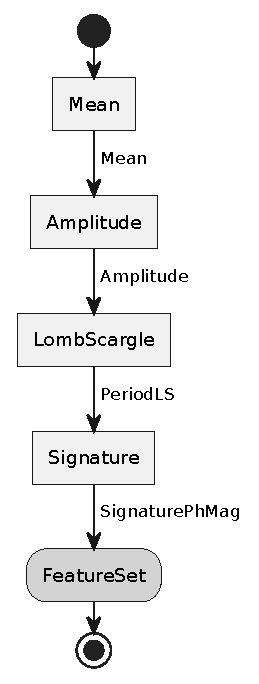
\includegraphics[width=.7\linewidth]{06_parallel/figures/sequential_ext.pdf}
    \caption{Plan de ejecución secuencial.}
\end{subfigure}%
\begin{subfigure}{0.6\textwidth}
    \centering
    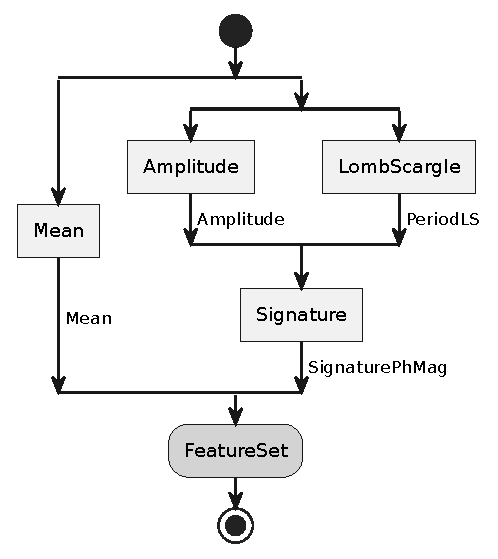
\includegraphics[width=.9\linewidth]{06_parallel/figures/parallel_ext.pdf}
    \caption{Grafo de ejecución paralelizado.}
\end{subfigure}

\caption{
    Esquema de ejecución de la extracción de características \texttt{Mean} y \texttt{SignaturePhMag} para el modelo secuencial y la nueva versión paralelizada. Las cajas representan los extractores individuales y las flechas indican el orden de ejecución. Una flecha que se divide en dos caminos distintos representa la paralelización de tareas, y las etiquetas en las flechas indican las características obtenidas por los extractores. Al final del proceso, se juntan todas las características extraídas en un \texttt{FeatureSet}, que se devuelve como salida.
}
\label{fig:execution_plans}
\end{figure}

La \autoref{fig:execution_plans} ilustra, a modo comparativo, el modelo secuencial de la versión original de \gls{feets} y el esquema paralelizado que implementamos en la nueva versión. Ambos modelos están aplicados al ejemplo de la extracción de \texttt{SignaturePhMag}, incorporando además la característica \texttt{Mean} a la selección, que no depende y no es dependencia de ninguna otra característica. En el enfoque secuencial, se observa que el plan de ejecución sigue una estructura con forma de cadena, ejecutando un solo extractor a la vez. En contraste, en el modelo paralelizado, se pueden identificar nodos independientes entre sí que se ejecutan en simultáneo, pero se conserva el orden de las dependencias cuando es necesario.

\section{Decisiones de diseño}

El ecosistema de Python ofrece diversas herramientas para la paralelización de tareas, pero para los propósitos de este proyecto optamos por el uso de la biblioteca \emph{Dask}\footnote{\url{https://www.dask.org/}} que se especializa en la ejecución de tareas distribuidas \citep{rocklin2015dask}. Entre los motivos detrás de esta elección se encuentran su facilidad de uso y su extensa documentación, pero también el hecho de que \emph{Dask} proporciona una \gls{api} robusta que permite modelar grafos de tareas para su ejecución en paralelo. Esta última funcionalidad es relevante porque funcionó como la base sobre la cual implementamos el grafo de ejecución utilizado en el nuevo modelo paralelizado de la extracción de características.

\emph{Dask} tiene también la ventaja de contar con distintos \emph{schedulers} internos que permiten decidir cómo se distribuyen las tareas según el \emph{hardware} disponible y la naturaleza del problema. De estos, nos interesan particularmente tres \emph{schedulers}:

\begin{itemize}
    \item \textbf{\texttt{synchronous}}. Ejecución secuencial, sin paralelismo.
    \item \textbf{\texttt{threads}}. Ejecución concurrente con \emph{multithreading}.
    \item \textbf{\texttt{processes}}. Ejecución paralelizada con \emph{multitprocessing}.
\end{itemize}

Todas las funcionalidades destinadas a la ejecución distribuida del modelo paralelizado las agrupamos en un nuevo módulo del sistema: \texttt{runner}. El módulo abstrae la comunicación con \emph{Dask}, definiendo una interfaz fija que proporciona los métodos necesarios para llevar a cabo la extracción paralelizada de características sin exponer el cómo se delegan las tareas a esta biblioteca.

La ventaja de tener el módulo \texttt{runner} con una interfaz fija es que, si al día de mañana se quiere reemplazar \emph{Dask} por otra biblioteca de ejecución distribuida, entonces solo hace falta reimplementar los métodos internos del módulo para que se comuniquen correctamente con este nuevo \emph{back end}. Estos cambios no deberían afectar el comportamiento externo de \texttt{runner}, lo que evita tener que hacer modificaciones en el resto del código, y además permite la ejecución de \emph{tests} automatizados para asegurar que el módulo funcione correctamente. \cleardoublepage
\chapter[\emph{Refactoring}: Modernizando feets]{
    \emph{Refactoring}: Modernizando \acrshort{feets}
}
\label{chapter:refactoring}

Además de paralelizar la extracción de características, con la nueva versión de \gls{feets} llevamos a cabo un proceso de refactorización que buscó modernizar el diseño general del sistema, proporcionar una \gls{api} más simple e intuitiva, y mejorar aún más el desempeño de los extractores. Este proceso de reingeniería, a su vez, dio lugar a la actualización del \emph{stack} tecnológico de la aplicación, la estandarización del estilo del código a lo largo y ancho del proyecto, y también al desarrollo de nuevas funcionalidades que consideramos útiles.

En las siguientes secciones del capítulo describiremos en detalle cada una de las modificaciones que implementamos en la nueva versión de \gls{feets}. Haremos hincapié en las decisiones de diseño que tomamos durante el proceso de desarrollo, y también hablaremos de las actualizaciones tecnológicas que llevamos a cabo en la infraestructura del proyecto.  

\section{Rediseño de extractores}

Uno de los cambios más importantes entre la versión original de \gls{feets} y la nueva implementación fue la completa renovación de la lógica de los extractores de características. El cambio consistió en volver a implementar la clase \texttt{Extractor} desde cero, que funciona como el modelo base detrás de todos los extractores del sistema.

La problemática que impulsó el rediseño de los extractores fue la complejidad que manejaba la metaclase \texttt{Extractor} la cual, como se explicó en el capítulo \autoref{chapter:feets}, mantenía una lógica compleja con uso de metaprogramación avanzada para asegurar el correcto comportamiento de las clases hijas. Tales técnicas estaban destinadas a asegurar que todas estas clases siguieran una interfaz común, definiendo métodos y atributos que deben ser implementados por todos los extractores y realizando validaciones específicas al momento de ejecución para verificar que el comportamiento sea el correcto.

En la nueva versión, reimplementamos desde cero la clase \texttt{Extractor} reemplazando el uso de la metaclase por el de una clase abstracta. Al igual que con la metaclase, esto nos permite especificar métodos y atributos obligatorios en la interfaz, pero lo hace de una manera más simple y fácil de entender sin la necesidad de técnicas de metaprogramación, buscando reducir drásticamente la complejidad de la clase. 

Además de emplear el uso de una clase abstracta, aprovechamos la reimplementación de la clase \texttt{Extractor} para también agregar nuevas funcionalidades a la interfaz y para eliminar algunos atributos redundantes. Las modificaciones se pueden visualizar en la figura \autoref{fig:extractor_class}, que compara los diagramas de clase de los extractores entre las versiones original y nueva de \gls{feets}.

\begin{figure}[!ht]
\centering
\begin{subfigure}{\textwidth}
    \centering
    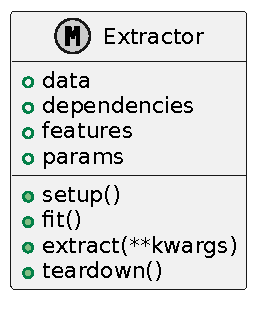
\includegraphics[width=.25\linewidth]{07_refactoring/figures/extractor_old.pdf}
    \caption{Diagrama de clases original}
\end{subfigure}

\begin{subfigure}{\textwidth}
    \centering
    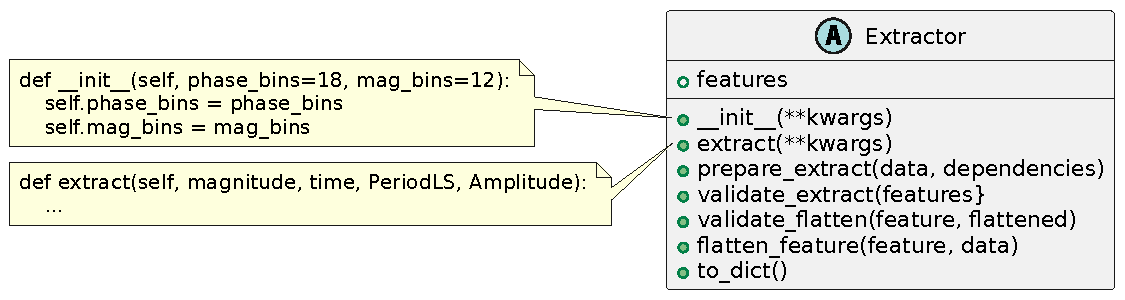
\includegraphics[width=\linewidth]{07_refactoring/figures/extractor_new.pdf}
    \caption{Nuevo diagrama de clases.}
\end{subfigure}

\caption{
    Diagramas de clase de \texttt{Extractor} antes y después de la nueva versión de \gls{feets}. Las anotaciones de la izquierda ejemplifican posibles implementaciones de los métodos señalados.
}
\label{fig:extractor_class}
\end{figure}

A continuación, hablaremos más en detalle sobre las distintas modificaciones que realizamos en la \gls{api} de extractores.

\begin{description}
    \item[Método de extracción] En primer lugar, los métodos \texttt{fit()} y \texttt{extract()} fueron reemplazados por un solo método abstracto, también con el nombre \texttt{extract()}, el cual debe ser implementado por todos los extractores con la lógica de extracción correspondiente.
    
    Los argumentos de entrada consisten de
    \begin{itemize}
        \item los vectores de datos de la \gls{lc} utilizados en el cálculo de las características,
        
        \item las características computadas por otros extractores que actúan como dependencias.
    \end{itemize}
    Cada uno de estos argumentos puede o bien ser obligatorio, requerido para la extracción; o ser opcional, con valores por defecto.

    \item[Método de inicialización] A diferencia de \texttt{fit()}, el nuevo método \texttt{extract()} no cuenta con parámetros extra para configuraciones opcionales. Esto es porque los parámetros de un extractor ya no se pasan como argumentos en el momento de su ejecución, sino que se asignan como atributos de la instancia durante la inicialización del objeto. 
    
    Ahora se permite la implementación de un método opcional \texttt{\_\_init\_\_()} personalizado en cada clase, el cual toma como argumentos de entrada los valores de los parámetros opcionales del extractor y los asigna a atributos de la clase durante su inicialización. Como requerimiento, los parámetros de un extractor son todos opcionales, por lo que se deben especificar en forma de \emph{keyword arguments} con valores por defecto.

    \item[Atributos redundantes] A simple vista es fácil notar que los atributos \texttt{data}, \texttt{dependencies} y \texttt{params} ya no se especifican en el cuerpo de la clase. Esto es porque todos estos valores se infieren automáticamente a partir de los argumentos que se especificaron en los nuevos métodos:

    \begin{itemize}
        \item Del método \texttt{\_\_init\_\_()} es posible determinar los parámetros opcionales del extractor (\texttt{params}).
        \item Los argumentos de \texttt{extract()} hacen posible inferir los datos de la \acrfull{lc} requeridos por el extractor (\texttt{data}), así como las dependencias de características (\texttt{dependencies}).
    \end{itemize}

    La inferencia de estos atributos se logra mediante introspección, una técnica de metaprogramación que permite al programa examinar su propia estructura en tiempo de ejecución. En este caso, se aplica en el momento de definición de la clase, permitiendo realizar validaciones y asegurar que los atributos inferidos respeten los formatos requeridos.

    \item[Normalización de características] Entre las nuevas funcionalidades de los extractores, incorporamos el método \texttt{flatten\_feature()} para normalizar las características computadas a valores unidimensionales. En particular, el método permite transformar diccionarios, listas o vectores de \emph{Numpy} a colecciones de valores escalares, de una sola dimensión.
    
    En caso de tratar con valores que no estén dentro de los tipos de datos soportados, el usuario puede expandir la lógica de este método en el extractor correspondiente para agregar la transformación adecuada para el tipo de datos necesario.

    \item[Persistencia] Con la intención de persistir el estado de los extractores entre ejecuciones, agregamos el método \texttt{to\_dict()} que provee una representación del estado interno del extractor en forma de un diccionario de Python. El diccionario incluye el nombre del extractor y los valores de los parámetros opcionales que se le asignaron al momento de incialización.

    \item[Método auxiliares] Por último, incorporamos algunos métodos destinados a acompañar comportamientos internos en la aplicación:

    \begin{itemize}
        \item \textbf{\texttt{prepare\_extract()}}: Confecciona y valida los argumentos del método \texttt{extract()} a partir de una selección de vectores de datos y de dependencias de características.
        \item \textbf{\texttt{validate\_extract()}}: Valida que la salida de  \texttt{extract()} produzca las características esperadas.
        \item \textbf{\texttt{validate\_flatten()}}: Valida que la salida de \texttt{flatten\_feature()} tenga el formato de una característica normalizada.
    \end{itemize}
\end{description}

El nuevo comportamiento de los métodos \texttt{extract()} e \texttt{\_\_init\_\_()}, así como la eliminación de definiciones de atributos \texttt{data}, \texttt{dependencies} y \texttt{params} del cuerpo de la clase, significó cambios mayores en la infraestructura de los extractores, lo que nos llevó a actualizar todos los extractores ya desarrollados en \gls{feets} para que adopten los nuevos requerimientos, y para que no rompan el comportamiento ya existente de la aplicación.

\section{Integración con \emph{LightCurve}}

En nuestra búsqueda por hacer que \gls{feets} sea más rápido, decidimos integrarla con una de las herramientas más modernas en la extracción de características de series temporales: \emph{LightCurve}. Desarrollada por \citet{malanchev2021lightcurve}, esta biblioteca se distingue por su enfoque en la eficiencia computacional, logrando tiempos de ejecución considerablemente menores en comparación con implementaciones tradicionales en Python. 

El secreto detrás de esta mejora radica en su implementación en Rust, un lenguaje de programación de bajo nivel diseñado para ofrecer alto rendimiento, pero sin comprometer la seguridad ni la concurrencia del código \citep{matsakis2014rust}. Rust permite ejecutar operaciones numéricas de forma optimizada, aprovechando técnicas avanzadas de paralelización y un uso eficiente de la memoria. Gracias a esto, \emph{LightCurve} supera muchas de las limitaciones de los extractores originales de \gls{feets}, proporcionando una ejecución más rápida y escalable, especialmente en el procesamiento de grandes volúmenes de datos.

En esta nueva versión, incorporamos todas las características de \emph{LightCurve} en \gls{feets}. Esto no solo amplía la lista de extractores disponibles para el análisis de series temporales, sino que también nos permitió reemplazar extractores preexistentes por sus versiones más eficientes, de lo posible. Así, en lugar de reinventar lo que ya está optimizado, optamos por una integración inteligente que nos permite combinar la flexibilidad de \gls{feets} con la velocidad de \emph{LightCurve}, logrando así lo mejor de ambos mundos.

Para hacer la integración lo más transparente posible, desarrollamos una nueva clase abstracta: \texttt{LightCurveExtractor}. Esta clase extiende el diseño de los extractores originales de \gls{feets} actuando como un puente entre ambas bibliotecas. A través de esta interfaz, cualquier extractor basado en \emph{LightCurve} se adapta automáticamente a la arquitectura de \gls{feets}, sin necesidad de cambios manuales ni configuraciones adicionales.

Uno de los principales desafíos en esta integración fue la diferencia en la representación de datos entre ambas bibliotecas. Mientras que \gls{feets} trabaja tradicionalmente con magnitudes aparentes, muchos de los extractores de \emph{LightCurve} operan directamente sobre flujos. El flujo es una medida física fundamental en astronomía, que representa la cantidad de luz recibida de un objeto en una determinada banda espectral y que, en muchos contextos, es más adecuada que la magnitud para ciertos tipos de análisis \citep{bessell2005standard}. Para hacer frente a esta diferencia, introdujimos dos nuevos tipos de datos en \gls{feets}, \texttt{flux} y \texttt{flux\_error}, asegurando así que los extractores de ambas bibliotecas puedan coexistir sin problemas dentro de la misma plataforma.

\section[Mejoras en la API]{
    Mejoras en la \gls{api}
}

Acompañando la reimplementación de los extractores, también incorporamos modificaciones en la \gls{api} del \texttt{FeatureSpace} para ofrecer nuevas funcionalidades a la herramienta y mejorar la flexibilidad de la extracción de características. Todas estas mejoras se detallan a continuación.

\begin{description}
    \item[Grupos de \acrlongplsp{lc}] Una de las principales molestias en el uso de \gls{feets} era que solo se podían extraer las características de una sola \gls{lc} a la vez. Bajo este modelo, si se querían analizar las mismas características entre varias \glspl{lc} distintas, hacía falta crear múltiples instancias de \texttt{FeatureSpace}, todas con la misma selección de características a extraer. Este proceso no solo puede ser tedioso si se quiere trabajar con varias curvas diferentes, sino que además puede llevar a inconsistencias cuando el usuario modifica la selección de uno de los tantos \texttt{FeatureSpace} inicializados y no tiene la consideración de realizar el mismo cambio en las demás instancias.
    
    Por esto, en la nueva versión de \gls{feets}, dimos soporte al procesamiento de múltiples \glspl{lc} en simultáneo mediante la instanciación de un único \texttt{FeatureSpace}, el cual define los conjuntos de características que se desean extraer para todas las curvas especificadas. 

    Aprovechando también la nueva implementación paralelizada del proceso de extracción, decidimos hacer que la ejecución de las distintas \glspl{lc} también sea paralelizada, por lo que no solo se reduce la cantidad de instancias de \texttt{FeatureSpace} que debe manejar el usuario, sino que además se aprovechan los recursos disponibles en el sistema para mejorar aún más el desempeño temporal de la aplicación. 
    
    \item[Selección automática de características] Otro de los cambios que implementamos fue una mejora al proceso de selección de características que ocurre previo al flujo de extracción. Para ser más específicos, incorporamos una nueva forma de inicializar el \texttt{Fea\-ture\-Space} que, partiendo de una \gls{lc}, permite seleccionar automáticamente todas las características que se pueden extraer a partir de los vectores de datos disponibles en la curva.
    
    El nuevo constructor, \texttt{from\_lc()}, funciona también para el caso en que se desea procesar más de una \gls{lc} a la vez. En este escenario, nos aseguramos que la selección final consista únicamente de las características extraíbles por todas las \glspl{lc} proporcionadas, teniendo en consideración que las distintas curvas no necesariamente presentan los mismos vectores de datos.
    
    Esta funcionalidad es muy útil porque facilita tremendamente la selección de todas las características posibles. Antes de este cambio, el usuario debía revisar las dependencias de datos de todos los extractores del sistema para determinar qué características eran alcanzables por la curva trabajada mientras que, en la nueva versión, todo este proceso se resuelve automáticamente con la llamada a un único método.

    \item[Persistencia de estados] Consideramos necesario el contar con un mecanismo para almacenar y reutilizar las configuraciones específicas de la extracción de características, por lo que añadimos la capacidad de exportar e importar objetos de la clase \texttt{FeatureSpace}.
    
    En la nueva interfaz, los usuarios son capaces de guardar instancias de un \texttt{FeatureSpace} en forma de diccionarios de Python o como archivos en los formatos \emph{JavaScript Object Notation} (JSON) \citep{bray2014json} o \emph{YAML Ain't Markup Language} (YAML) \citep{ben2009yaml}; todo esto, mediante los nuevos métodos \texttt{to\_dict()}, \texttt{to\_json()} y \texttt{to\_yaml()}, respectivamente. 
    
    A partir de las estructuras exportadas, los usuarios pueden hacer uso de los constructores \texttt{from\_dict()} (para diccionarios), \texttt{from\_json()} (archivos JSON) y \texttt{from\_yaml()} (archivos YAML), que les permiten restaurar el estado del \texttt{FeatureSpace} original con todas las configuraciones guardadas. Estos estados incluyen las características seleccionadas para ser extraídas, las instancias parametrizadas de los extractores, los datos requeridos por la selección de características, y algunas opciones particulares para ajustar la extracción paralelizada.
    
    La gestión de las tareas de lectura y escritura de archivos las desarrollamos en un nuevo módulo del sistema, \texttt{io}, quien además se encarga de la correcta codificación de las configuraciones a los distintos formatos permitidos.

    \item[Interfaz de características] Por último, otra de las principales mejoras de la \gls{api} fue la introducción de la clase \texttt{Features}, que redefine la forma en que se exploran los resultados de la extracción de características. Con una interfaz más robusta y una funcionalidad expandida, \texttt{Features} viene a reemplazar la clase \texttt{FeatureSet}, implementada en la versión original de \gls{feets}.

    El objetivo principal de la clase \texttt{Features} es el de manejar la representación de las características resultantes del procesamiento de una o varias \glspl{lc} para su análisis posterior. Una instancia de esta clase se puede explorar de dos formas distintas:
    \begin{itemize}
        \item como un arreglo de \glspl{lc}, donde cada elemento consiste de un diccionario con los resultados de todas las características de una de las curvas procesadas; o bien,
        \item como un objeto, en el que cada atributo representa una de las características seleccionadas, y su valor es un arreglo con los respectivos resultados obtenidos en cada \gls{lc}.
    \end{itemize}

    Con la intención de usar esta clase para el análisis de características, implementamos también la capacidad de representar los datos en forma de un \texttt{DataFrame} de \emph{Pandas}\footnote{\url{https://pandas.pydata.org/}}, mejorando también la interoperabilidad de \gls{feets} dentro del ecosistema de Python. Con esto en mente, la clase \texttt{Features} puede servir como base para futuras herramientas de análisis, aprovechando su estructura actual para modelar, por ejemplo, una forma de proporcionar un gráfico representativo de cada característica.
\end{description}

    \section{Cambios menores}

Además de las mejoras fundamentales introducidas en esta nueva versión de \gls{feets}, realizamos una serie de optimizaciones y actualizaciones que elevan significativamente la calidad, compatibilidad y usabilidad del proyecto. Estos cambios, aunque menores en términos de implementación, impactan en la experiencia de los usuarios y en la eficiencia del código, asegurando que \texttt{feets} se mantenga alineado con las mejores prácticas y tecnologías más avanzadas. A continuación, detallamos las principales mejoras incorporadas:

\begin{description}
    \item[Compatibilidad] Actualizamos los requisitos de \gls{feets} y eliminamos por completo el soporte para Python 2. Ahora, \texttt{feets} es compatible con las versiones de Python 3.10 a 3.13 inclusive, lo que permite aprovechar las últimas optimizaciones y nuevas características del lenguaje.

    Entre las novedades más destacadas, Python 3.13 introduce un modo de ejecución experimental sin el \acrfull{gil}, haciendo opcional su uso y permitiendo \emph{full-threading} en escenarios altamente paralelizables \citep{gross2023nogil}. Si bien esta funcionalidad aún está en sus primeras etapas, su desarrollo representa un cambio radical en la evolución del lenguaje y abre nuevas posibilidades para mejorar el rendimiento de bibliotecas científicas y de análisis de datos. A medida que esta tecnología madure en futuras versiones, \texttt{feets} estará preparado para aprovechar todo su potencial.

    \item[Actualización de bibliotecas] En la nueva versión, renovamos por completo las dependencias principales para garantizar estabilidad, seguridad y acceso a las últimas innovaciones en \emph{Data Science}. Destacan particularmente las mejoras introducidas en:
    \begin{itemize}
        \item \emph{AstroPy} 7.0, que incorpora múltiples optimizaciones en el manejo de datos astronómicos, nuevas herramientas para análisis de series temporales y un rendimiento significativamente mejorado en operaciones comunes \citep{astropy2013astropy, astropy2018astropy, astropy2022astropy}.
        \item \emph{NumPy} 2.2.0, que introduce mejoras sustanciales en la eficiencia de operaciones matriciales, reducción del consumo de memoria y una mejor integración con las últimas versiones de Python \citep{harris2020array}. Estas optimizaciones son fundamentales para el procesamiento de grandes volúmenes de datos en \texttt{feets}, mejorando la velocidad de extracción de características sin comprometer la precisión.
    \end{itemize}

    \item[Estilo del código] La legibilidad y la calidad del código son fundamentales en un proyecto de código abierto, por lo que reforzamos el cumplimiento del estándar PEP 8 \citep{van2001pep8} y automatizamos el ajuste del formato con herramientas especializadas. Utilizamos:
    \begin{itemize}
        \item \emph{Flake8}\footnote{\url{https://flake8.pycqa.org/en/latest/}}, para garantizar un análisis estático del código y detectar posibles errores antes de su ejecución.
        \item \emph{Black}\footnote{\url{https://black.readthedocs.io/en/stable/}}, para asegurar un estilo consistente, facilitando la lectura del código y simplificando la colaboración entre varios desarrolladores.
    \end{itemize}

    \item[Ampliación de documentación y \emph{testing}] Para garantizar que los usuarios puedan aprovechar al máximo las nuevas capacidades de \texttt{feets}, expandimos y refinamos la documentación oficial de la herramienta. Ahora incluye ejemplos prácticos de uso, mejores explicaciones sobre la estructura de la \gls{api} y un tutorial actualizado con las nuevas funcionalidades incorporadas.

    Además, revisamos y actualizamos la \emph{test suite} para reflejar todos los cambios en la \gls{api}, asegurando una cobertura completa de las nuevas funcionalidades. Esta estrategia no solo mejora la confiabilidad del software, sino que también facilita futuras expansiones del proyecto sin comprometer la estabilidad del código base.
\end{description} \cleardoublepage
\chapter{Resultados}
\label{chapter:resultados}

Con el objetivo de evaluar si la nueva versión de \gls{feets} logra efectivamente mitigar las limitaciones identificadas en su versión original, realizamos una evaluación exhaustiva centrada tanto en el desempeño computacional como en la calidad estructural del código.

Por un lado, analizamos los tiempos de ejecución del sistema bajo distintas configuraciones experimentales, con el fin de determinar el impacto de la paralelización y la incorporación de nuevas funcionalidades. Por el otro, examinamos la evolución de la mantenibilidad del código mediante técnicas de análisis estático, con el propósito de cuantificar los efectos de las mejoras implementadas en términos de calidad. A continuación, presentamos en detalle los análisis realizados y los resultados obtenidos.

\section{Comparación de tiempos de ejecución}

Para evaluar el desempeño del nuevo modelo de extracción paralelizado, medimos sistemáticamente los tiempos de ejecución del proceso de extracción de características a lo largo de una serie de experimentos controlados. En cada experimento, generamos aleatoriamente un conjunto de una o más \glspl{lc} periódicas, simuladas al azar, que luego utilizamos como entrada para el proceso de extracción. Repetimos las pruebas variando los siguientes parámetros:

\begin{enumerate}
    \item \textbf{Longitud:} Número total de observaciones en cada una de las \glspl{lc} simuladas. Las longitudes variaron entre 30, 100, 300 y 1000 observaciones.
    
    \item \textbf{Tamaño:} La cantidad de \glspl{lc} simuladas que se procesaron en simultáneo. Probamos con tamaños de 1, 50, 100, 500 y 1000 \glspl{lc}.

    \item \textbf{Estrategia:} La configuración utilizada por el \emph{scheduler} de \emph{Dask} para distribuir las tareas. Como mencionamos en el \autoref{chapter:parallel}, nos interesaron tres \emph{schedulers} preestablecidos: \texttt{synchronous} (sin paralelismo), \texttt{threads} (\emph{multithreading}) y \texttt{processes} (\emph{multiprocessing}). 
\end{enumerate}

Al combinar las distintas configuraciones de los tres parámetros, obtenemos 60 experimentos distintos. Para cada uno de ellos, realizamos diez iteraciones independientes, generando en cada repetición un nuevo conjunto de \glspl{lc} simuladas. En total, se llevaron a cabo 600 casos de prueba, en los cuales medimos el tiempo de ejecución del proceso completo de extracción en dos escenarios distintos:

\begin{enumerate} 
    \item \textbf{Selección completa:} Abarcando todas las características disponibles en la nueva versión de \gls{feets}, incluyendo las que incorporamos mediante la integración con \textit{LightCurve}. 
    
    \item \textbf{Selección reducida:} Limitada únicamente a las características que ya estaban presentes en versiones anteriores de la herramienta.
\end{enumerate}

Las mediciones fueron llevadas a cabo en la supercomputadora Serafín, provista por la \unc{}. Cada caso de prueba se ejecutó en una unidad de cómputo con las siguientes características:

\begin{description}
    \item[CPU] -- $\SI{2.4}{\giga\hertz}$ AMD EPYC\texttrademark{} 7532 ($2\times32$ núcleos, 64 hilos, $\SI{256}{\mega\byte}$ de caché, hasta $\SI{3.3}{\giga\hertz}$).
    \item[RAM] -- $\SI{128}{\gibi\byte}$ DDR4 SDRAM ($16 \times \SI{8}{\gibi\byte}$, $\SI{3200}{\mega\hertz}$).
    \item[OS] -- Rocky Linux 8.8 con Linux Kernel 4.18.
    \item[\emph{Software}] -- \textit{Python} 3.13.2, \textit{NumPy} 2.2.4, \textit{SciPy} 1.15.2, \textit{AstroPy} 7.0.1, \textit{StatsModels} 0.14.4, \textit{Dask} 2025.3.0 y \textit{Light\-Curve} 0.10.2.
\end{description}

\subsection{Análisis de resultados}

\begin{figure}[!ht]
\centering
\begin{subfigure}{\textwidth}
    \centering
    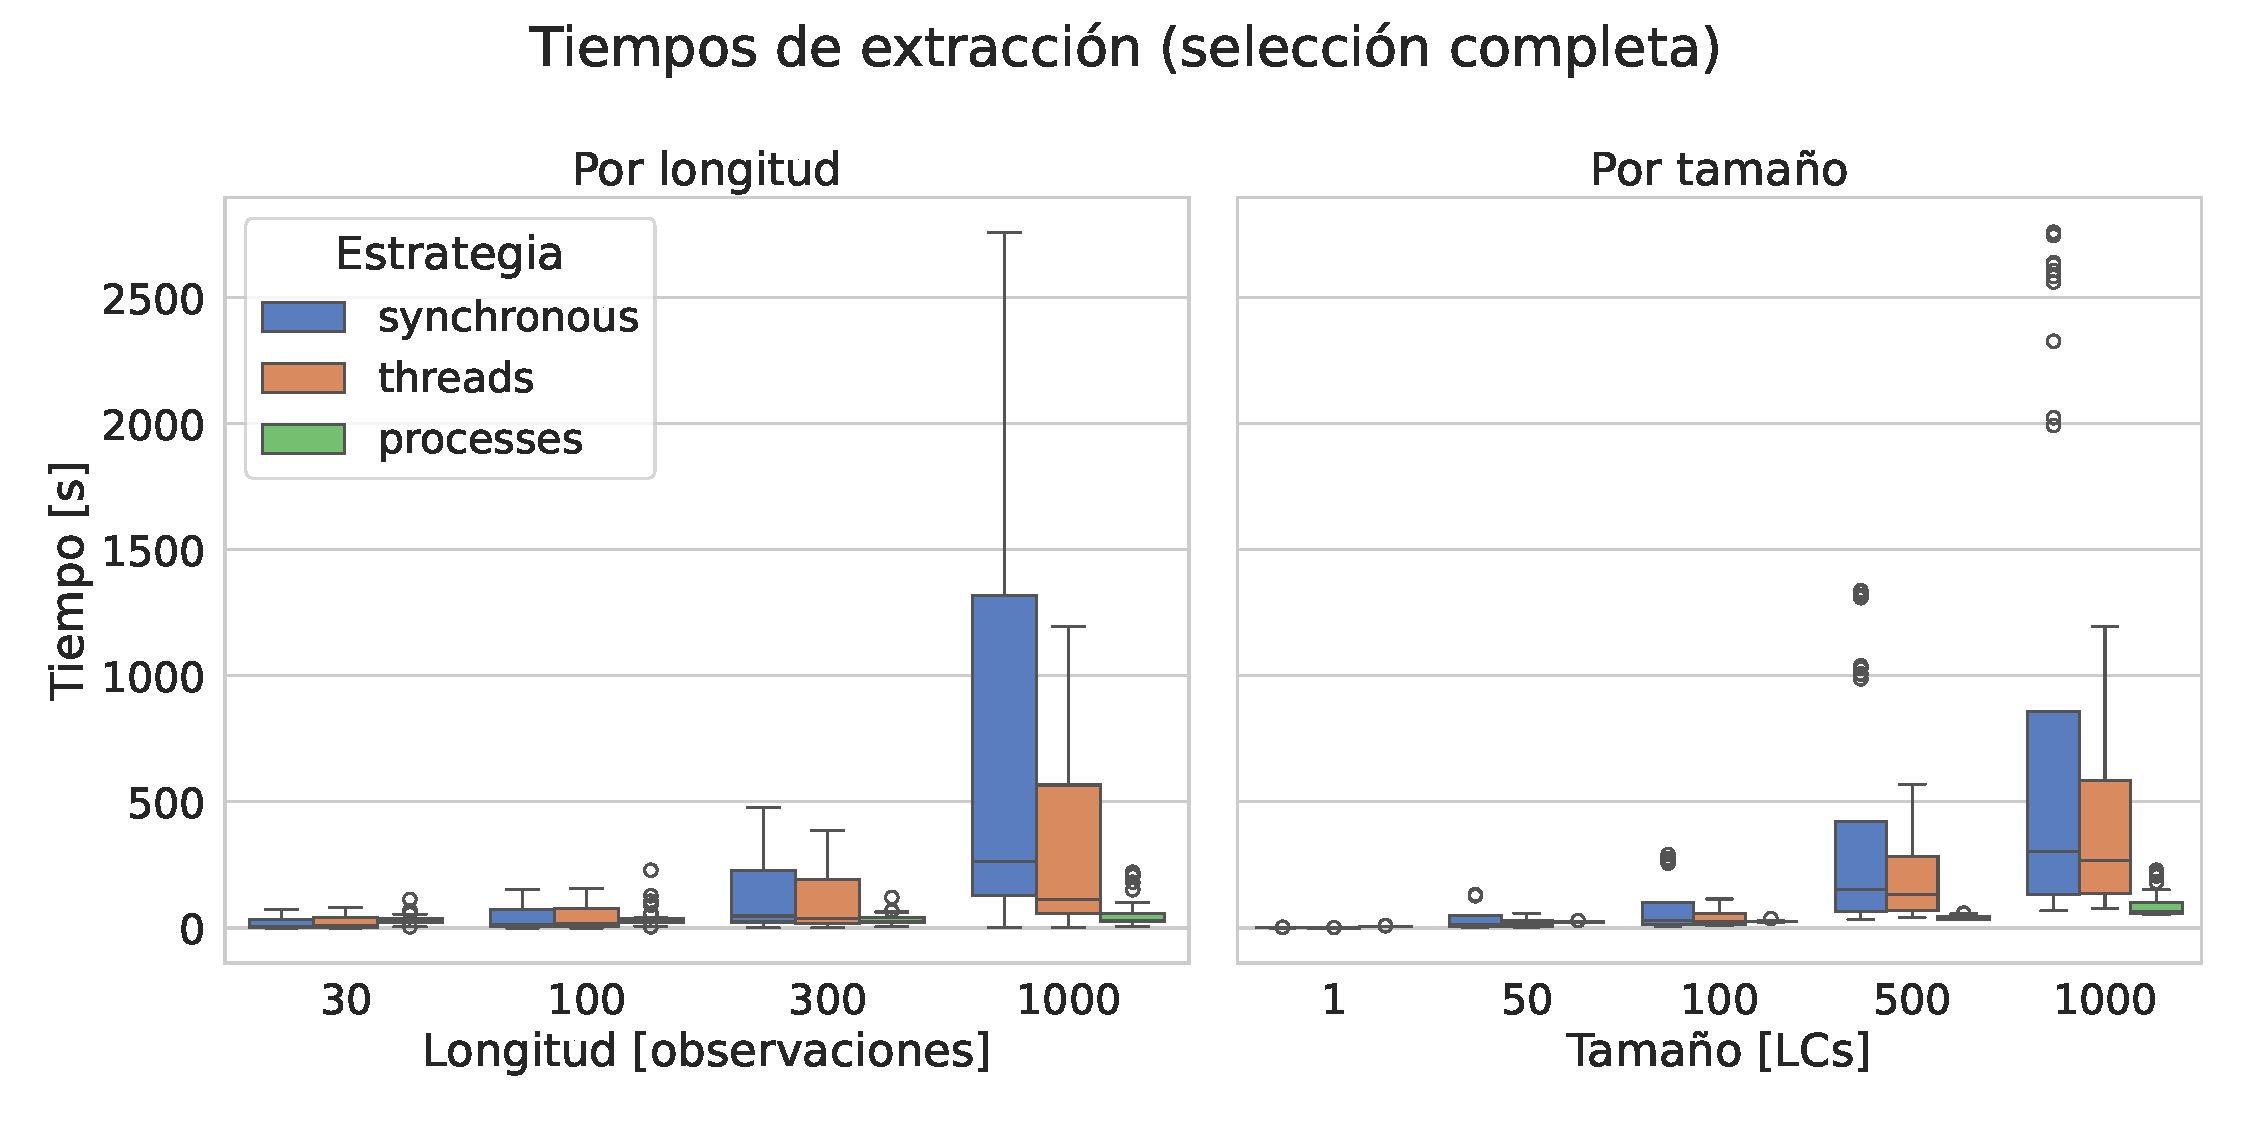
\includegraphics[width=\linewidth]{08_resultados/figures/01_analysis_all.pdf}
    \caption{Tiempos de extracción para la selección completa}
    \label{fig:analysis_all}
\end{subfigure}

\begin{subfigure}{\textwidth}
    \centering
    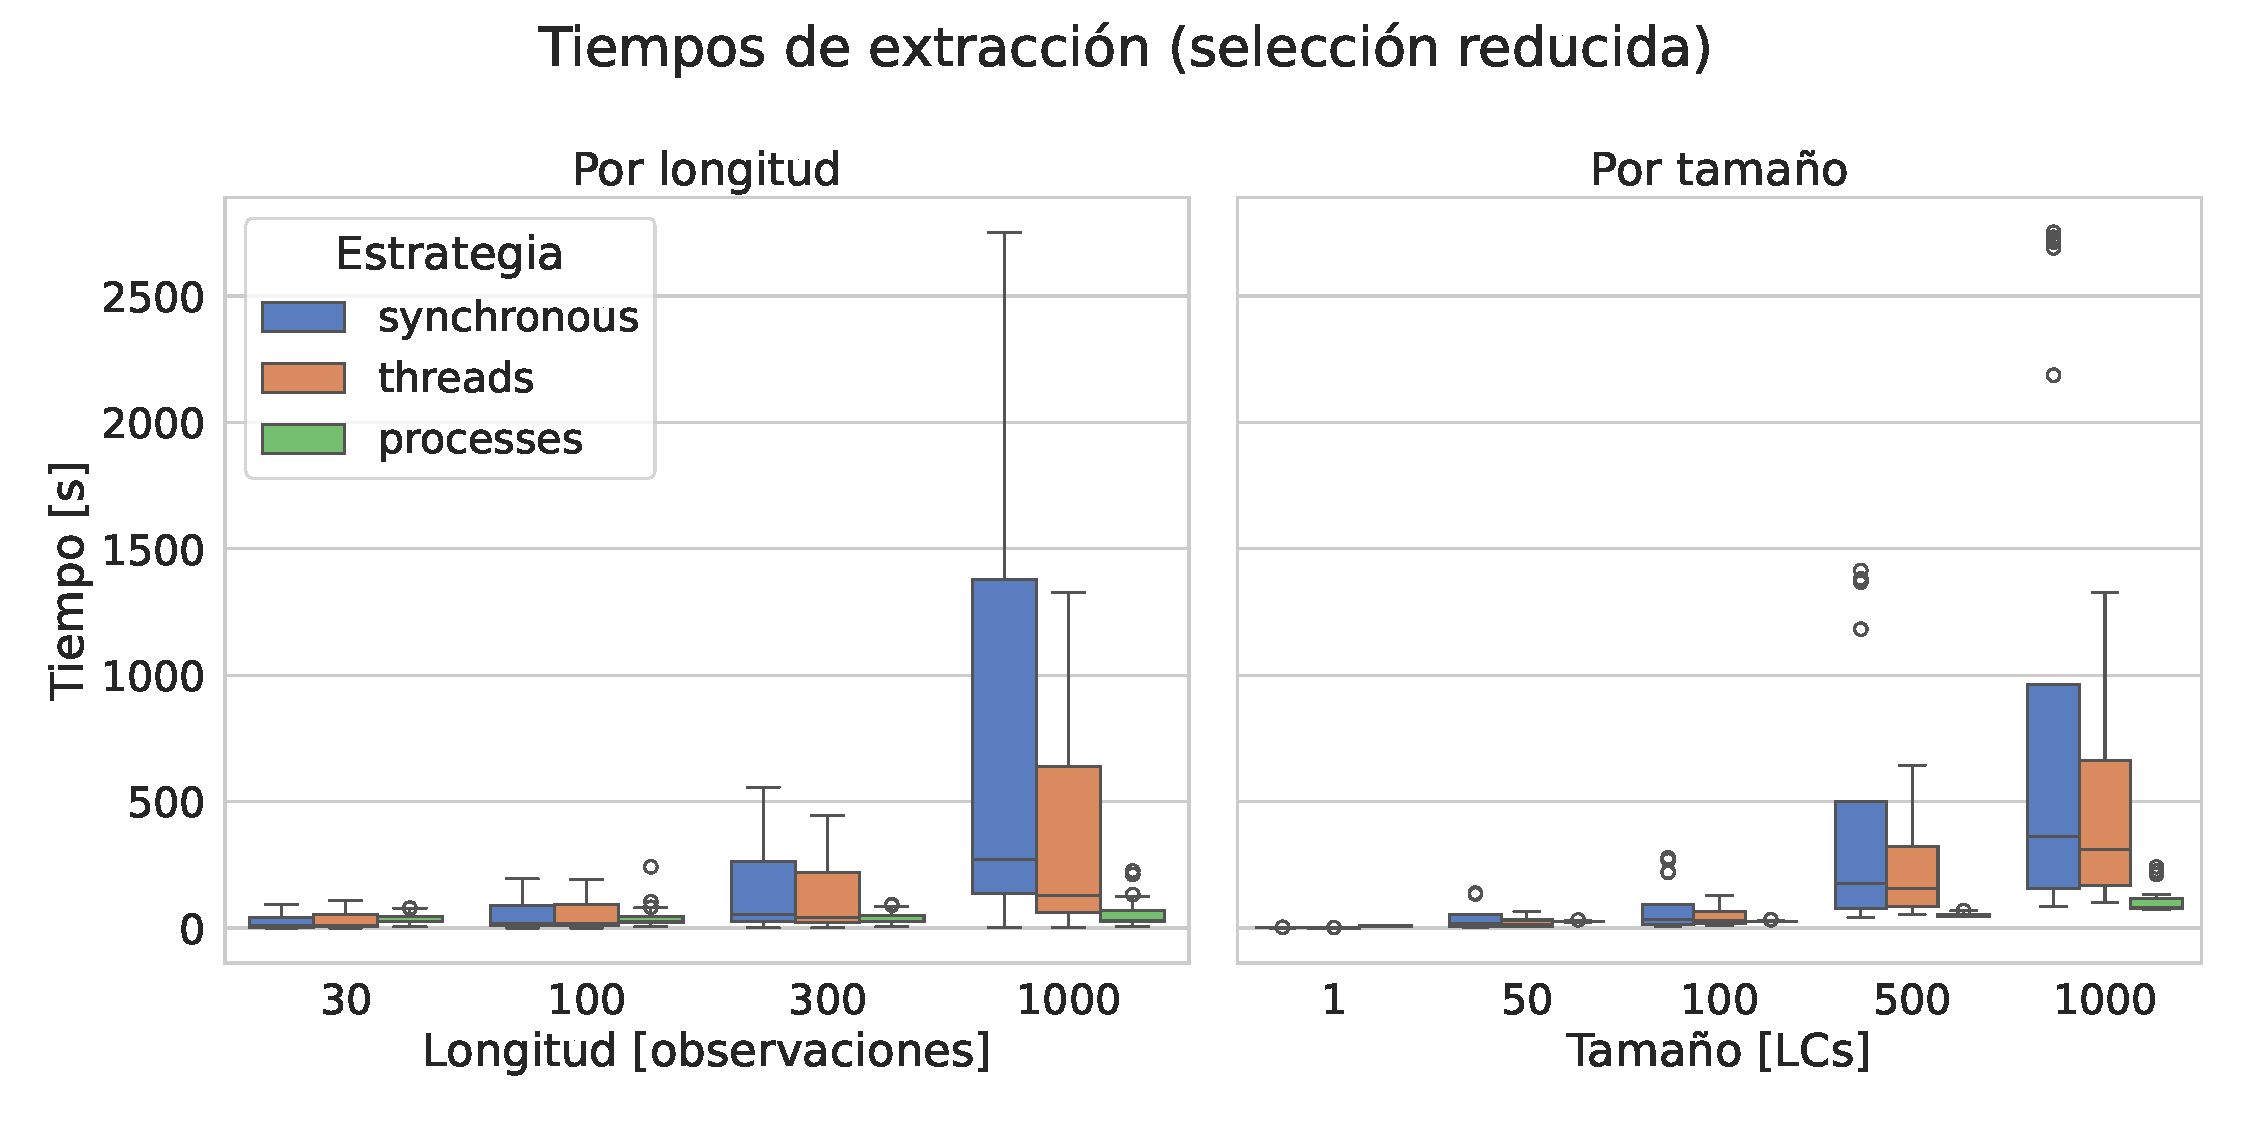
\includegraphics[width=\linewidth]{08_resultados/figures/01_analysis_exclude.pdf}
    \caption{Tiempos de extracción para la selección reducida}
    \label{fig:analysis_exclude}
\end{subfigure}

\caption{
    Evolución de los tiempos de extracción obtenidos para los 600 casos de prueba. Se visualizan dos conjuntos de gráficos por cada figura: uno en función a la longitud de las \glspl{lc} simuladas, y el otro en función a la cantidad de \glspl{lc} procesadas en simultáneo. Cada línea de color representa una estrategia del \emph{scheduler} de \emph{Dask} diferente.
}
 \label{fig:analysis}
\end{figure}

Los resultados obtenidos se resumen en las Figuras~\ref{fig:analysis_all} y~\ref{fig:analysis_exclude}, que presentan los tiempos correspondientes a la extracción tanto de todas las características del sistema como de la selección reducida, respectivamente. En términos generales, observamos que en los dos escenarios los tiempos de ejecución aumentan tanto con la longitud de las curvas como con el tamaño del conjunto. Esta relación era esperable, ya que un mayor volumen de datos implica un mayor esfuerzo computacional.

Al observar el comportamiento de las distintas estrategias de planificación, notamos que en los casos de menor volumen de datos (tanto el de menor longitud de observaciones como el de menor cantidad de \glspl{lc}) todas las estrategias muestran un rendimiento muy similar. En particular, \texttt{synchronous} suele ser ligeramente más rápida en esos escenarios, posiblemente porque los costos asociados a la creación, distribución y comunicación de tareas paralelas superan los beneficios del paralelismo en situaciones de baja carga. A medida que el volumen de los datos aumenta, \texttt{synchronous} muestra una tendencia clara a producir tiempos de ejecución progresivamente más altos, estableciéndose como la estrategia que peor escala. Este comportamiento evidencia la idea de que el paralelismo contribuye de manera efectiva a reducir los tiempos de extracción en contextos con mayor demanda.

Si nos centramos ahora en las dos estrategias concurrentes, observamos que \texttt{threads} presenta una mejora clara respecto de \texttt{synchronous}, especialmente en configuraciones de carga media. No obstante, \texttt{processes} demuestra ser consistentemente más eficiente que \texttt{threads}, con una ventaja considerable cuando la carga de datos es más elevada. Esta diferencia sugiere que el \emph{multiprocessing} permite un uso mucho más efectivo de los recursos disponibles con respecto al \emph{multithreading}, probablemente al evitar las limitaciones impuestas por el \gls{gil} de Python.

Cabe señalar que Dask ofrece otros \emph{schedulers} además de los tres evaluados, incluyendo el \texttt{distributed}, un planificador altamente configurable que permite ejecutar tareas en clústeres de múltiples máquinas o entornos con recursos heterogéneos. Explorar el comportamiento del sistema bajo esta configuración podría resultar especialmente interesante para escenarios con grandes volúmenes de datos o requerimientos de alta disponibilidad, y constituye una posible línea de trabajo futura.

Ahora bien, al comparar los escenarios de extracción completa y reducida, notamos que los tiempos de ejecución son similares en todos los casos, pero que en algunas configuraciones la extracción completa muestra tiempos ligeramente menores. Este resultado es especialmente interesante, ya que ambos escenarios se probaron sobre los mismos conjuntos de \glspl{lc}, siendo la única diferencia entre los dos la selección de características extraídas.

Una posible explicación para la mejora de la extracción completa es que las nuevas características incorporadas provienen de la integración con \textit{LightCurve}, la cual implementa sus funciones internas de forma altamente optimizada. Es posible que la forma en que estas operaciones están estructuradas y que interactúan con el planificador de tareas de \emph{Dask} favorezcan a una mejor distribución de carga o a una ejecución más eficiente en paralelo. En ese sentido, aunque se estén calculando más características, el sistema podría estar aprovechando mejor los recursos disponibles gracias al diseño eficiente de la implementación subyacente.

En cualquier caso, las diferencias de tiempo entre los dos escenarios son mínimas y no permiten concluir que una configuración sea sistemáticamente más rápida que la otra, pero sí permiten afirmar que la inclusión de nuevas características no introduce un costo computacional significativo. El rendimiento del sistema se mantiene estable independientemente del conjunto de características utilizadas, lo que refleja una implementación robusta, eficiente y bien integrada.

\section{Análisis estático de código}

Además de optimizar el desempeño de \gls{feets} para la extracción de características, otro de los objetivos centrales de este trabajo fue mejorar la calidad interna del código, es decir, su claridad, modularidad y facilidad de mantenimiento. Para evaluar este aspecto, aplicamos un enfoque de análisis estático, centrado en el cálculo del \acrfull{mi} del sistema a lo largo del tiempo.

\subsection{Análisis de resultados}

Para realizar el análisis, optamos por la herramienta \emph{Wily}\footnote{\url{https://wily.readthedocs.io/en/latest/}}, una biblioteca de Python que permite monitorear la evolución histórica de distintas métricas de calidad del código fuente. \emph{Wily} analiza cada revisión en el historial de Git del proyecto, generando un seguimiento detallado de métricas de complejidad y de tamaño y, en particular, el \gls{mi}.

Como vimos en el \autoref{chapter:antecedentes}, existen varias formas distintas para determinar el \gls{mi}, pero este cálculo normalmente involucra cuatro métricas fundamentales:

\begin{itemize}
    \item Comlejidad ciclomática (\acrshort{cc})
    \item Volumen de Halstead (\acrshort{hv})
    \item Líneas de código (\acrshort{loc})
    \item Porcentaje de comentarios (\acrshort{poc})
\end{itemize}

En nuestro caso, \emph{Wily} utiliza internamente la biblioteca \emph{Radon}\footnote{\url{https://radon.readthedocs.io/en/latest/}} para determinar el \gls{mi}, cuyo cálculo se basa en las variantes del \gls{sei} \citep{bray1997c4} y la de Visual Studio \citep{microsoft2025mi} para obtener la siguiente fórmula: \[
    \max \Bigg[
        0, \;
        \frac{100}{171}
        \Big(
            171 - 5.2\ln{\text{V}} - 0.32\text{CC}
            - 16.2\ln{\text{LOC}} + 50 \sin{\sqrt{2.4 \text{POC}}}
        \Big)
    \Bigg]
\]
Este cálculo pondera negativamente la complejidad y el tamaño del código, y positivamente la presencia de comentarios, dejándolo en un rango de valores entre 0 y 100. Cuanto más alto sea el puntaje, mayor será la mantenibilidad del archivo.

Un aspecto técnico importante a mencionar es que la herramienta \emph{Radon}, por defecto, no considera las cadenas de documentación (\emph{docstrings}) como parte de los comentarios, sino que las contabiliza como líneas de código normales. Esto genera una disminución significativa del \gls{mi} en módulos bien documentados, lo cual resulta en una aparente contradicción: una mejora en la legibilidad y comprensión del código penaliza su mantenibilidad según el puntaje. Para resolver esta paradoja, optamos por configurar \texttt{radon} de modo que los \emph{docstrings} sean tratados como comentarios. Consideramos que esta decisión refleja de manera más justa el impacto positivo de la documentación sobre la calidad y sostenibilidad del sistema.

\subsection{Resultados y análisis}

\begin{figure}[!ht]
    \centering
    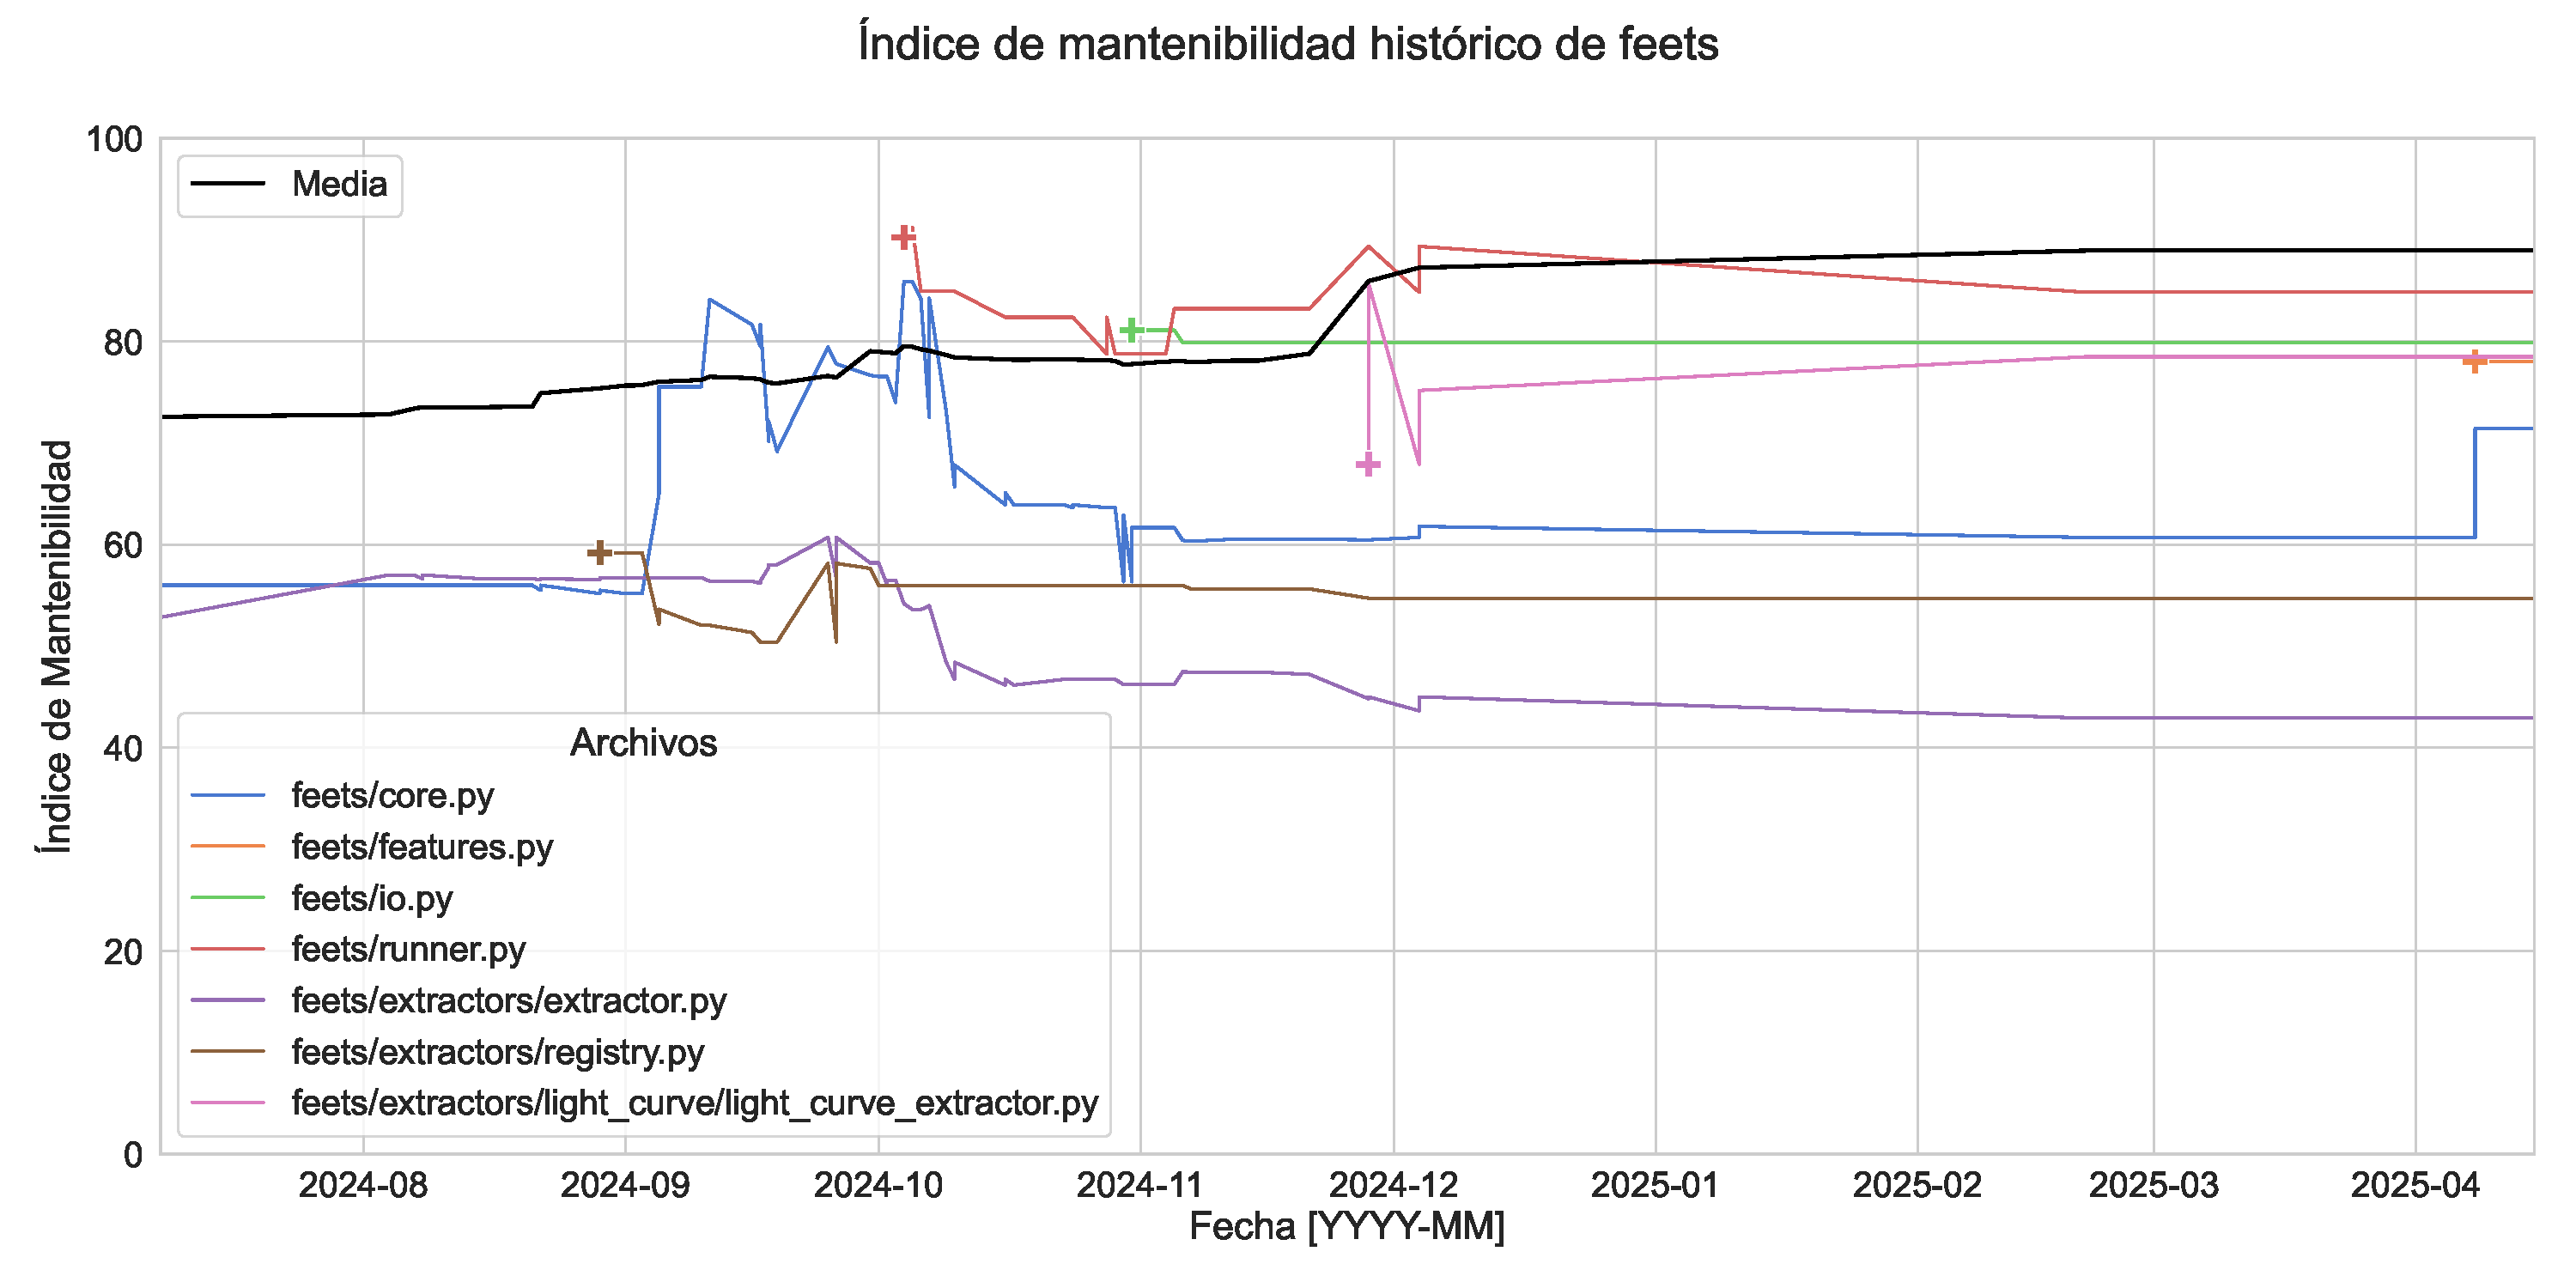
\includegraphics[width=\linewidth]{08_resultados/figures/MI_feets.pdf}
    \caption{
        Evolución del \gls{mi} de \gls{feets} durante el desarrollo de la nueva versión. La curva en negro representa la media del \gls{mi} considerando todos los archivos del sistema. Las líneas de colores, en cambio, muestran el \gls{mi} de algunos archivos individuales, seleccionados por su relevancia funcional, usando el símbolo \texttt{+} para marcar el momento en que se incorporaron al control de versiones.
    }
    \label{fig:mi}
\end{figure}

La \autoref{fig:mi} presenta la evolución del \gls{mi} a lo largo del proceso de modernización de \gls{feets}. Esta visualización permite identificar tendencias generales y también comportamientos específicos de ciertos módulos relevantes.

El valor medio del \gls{mi} global (representado por la curva negra) evidencia una ascendencia consistente en la mantenibilidad del sistema. Notamos un incremento de $72.59$ a $88.94$ puntos en el período analizado, reflejando una mejora sostenida en la calidad del código fuente de \gls{feets}. Desde una perspectiva técnica, este crecimiento puede atribuirse a prácticas de refactorización, modularización y reorganización de componentes, que derivaron en una base de código más clara y fácil de mantener.

Entre los archivos relevantes del proyecto, podemos notar algunas tendencias claras:

\begin{itemize}
    \item El módulo \texttt{feets/core.py} mostró un crecimiento destacado en su \gls{mi}; más aún, su curva muestra picos ascendentes en el momento en que se agregaron los módulos \texttt{feets/runner.py}, \texttt{feets/io.py} y \texttt{feets/features.py}. Este comportamiento es coherente con los cambios realizados en la nueva versión, pues gran parte de la lógica de \texttt{feets/core.py} fue externalizada a los módulos mencionados, sugiriendo que la separación de responsabilidades tuvo un impacto positivo en la mantenibilidad del código.

    \item En contraposición, el archivo \texttt{feets/extractors/extractor.py} experimentó una disminución gradual en su \gls{mi}. Esta tendencia también es esperable, ya que los nuevos extractores introdujeron funcionalidades adicionales, validaciones más complejas y capacidad de ejecución en paralelo, lo cual incrementó inevitablemente la complejidad del código y, por lo tanto, redujo su mantenibilidad.

    \item El archivo \texttt{feets/lightcurve/light\_curve\_extractor.py} mantuvo un \gls{mi} elevado desde su incorporación, lo cual sugiere que fue diseñado desde el inicio con buenas prácticas y una estructura clara. Este módulo actúa como puente entre los extractores de características de \gls{feets} y los de \textit{LightCurve}, por lo que su buen desempeño en términos de mantenibilidad indica que la integración fue realizada sin comprometer la calidad estructural del sistema.
\end{itemize}

A pesar de las variaciones individuales, el \gls{mi} se mantuvo en general en valores altos para los módulos relevantes, con puntajes superiores a los 60 puntos en la mayoría de los casos. Las excepciones más notorias fueron \texttt{feets/ex\-trac\-tors/re\-gis\-try.py} y \texttt{feets/extractors/extractor.py}, que mantuvieron puntajes más bajos y representan áreas donde aún queda margen de mejora en términos de claridad, modularidad y simplicidad estructural.

En conjunto, los resultados muestran que el sistema no solo creció funcionalmente, sino que lo hizo con una mejora tangible en su calidad interna. El análisis histórico del \gls{mi} permite afirmar que las decisiones de diseño y refactorización aplicadas durante el desarrollo tuvieron un impacto positivo en la mantenibilidad del código.

\section{Conclusiones del capítulo}

Juntando los resultados obtenidos a lo largo del capítulo, observamos que no solo la modernización de \gls{feets} llevó a mejoras significativas en los tiempos de ejecución de la herramienta, sino que también logró hacerlo sin comprometer la mantenibilidad global del sistema. En conjunto, estos hallazgos confirman que la nueva versión de \texttt{feets} representa un avance tanto en rendimiento como en calidad técnica. \cleardoublepage
\chapter{Conclusiones}
\label{chapter:conclusiones}

En este trabajo llevamos a cabo una refactorización integral de la herramienta \gls{feets} para mejorar su desempeño en contextos de grandes volúmenes de datos, como los planteados por relevamientos astronómicos modernos tales como el \gls{vvv} o \gls{macho}. El nuevo modelo de extracción paralelizado con \textit{Dask} eliminó el cuello de botella presente en la implementación secuencial de la versión original, demostrando tiempos de ejecución significativamente más cortos y escalando adecuadamente ante flujos de datos masivos, propios de la astronomía contemporánea.

Durante el proceso de refactorización logramos, además, mejorar la arquitectura del sistema y estandarizar el código con buenas prácticas de ingeniería del \emph{software}, resultando en un mayor \acrlongsp{mi} global y elevando la calidad interna del proyecto. También modernizamos el \emph{stack} tecnológico de la herramienta, siguiendo la adopción de versiones modernas de Python y la integración de la biblioteca \textit{LightCurve}, que nos permitió incorporar nuevos extractores de características eficientes sin comprometer el desempeño de la aplicación.

Aprovechando las mejoras tanto en el rendimiento como en la calidad del \emph{software}, realizamos cambios a la \gls{api} para también extender su funcionalidad. La nueva implementación de \gls{feets} permite procesar múltiples \glspl{lc} de manera simultánea, simplifica el desarrollo de nuevos extractores mediante un \emph{framework} más eficiente, e introduce una estructura de datos optimizada para la visualización y el análisis posterior de las características extraídas.

Como resultado, la nueva versión de \textit{feets} convierte a la herramienta en una solución robusta, rápida y moderna, que no solo supera las limitaciones de su versión anterior, sino que también está preparada para seguir evolucionando ante los desafíos que presenta el análisis de series temporales en la era del \emph{Big Data}.

\section{Trabajo a futuro}

Cuando evaluamos los tiempos de cómputo para distintas estrategias de planificación, consideramos que otra dirección prometedora sería evaluar el comportamiento del sistema utilizando el planificador \texttt{distributed} que ofrece \textit{Dask}. Este \emph{scheduler}, altamente configurable, permite ejecutar tareas en clústeres distribuidos o en entornos heterogéneos, y podría ofrecer mejoras significativas en escenarios con grandes volúmenes de datos o requerimientos de alta disponibilidad. Su exploración permitiría comprender mejor los límites de escalabilidad del sistema y ajustar dinámicamente la estrategia de ejecución según la demanda computacional.

Por otro lado, el análisis estático del código reveló un \gls{mi} bajo en los módulos encargados de la lógica base de los extractores y del registro de todos los extractores del sistema. Este resultado era esperable dado que la clase abstracta \texttt{Extractor}, responsable del comportamiento general de todos los extractores, aumentó en complejidad con el objetivo de simplificar la implementación de nuevos extractores. A pesar de esto, esta observación señala áreas concretas del sistema donde sigue siendo necesario mejorar la estructura interna del código y facilitar su mantenimiento a largo plazo.

Otra línea de trabajo futuro consiste en extender la funcionalidad de persistencia actualmente limitada a los formatos JSON y YAML. Incorporar compatibilidad con otros formatos de serialización o con bases de datos livianas como \textit{SQLite} podría favorecer la interoperabilidad con otros sistemas y optimizar los flujos de trabajo en distintos contextos de análisis. Siguiendo esta línea de pensamiento, consideramos viable la posibilidad de abstraer el \emph{back end} destinado a la ejecución paralela, dando lugar a la posibilidad de reemplazar \textit{Dask} por otras bibliotecas como \textit{Ray} o \textit{Joblib}. Así, sería posible adaptar la estrategia de paralelización a las necesidades específicas del entorno de ejecución sin modificar la lógica de alto nivel de la aplicación.

Por último, otra funcionalidad que consideramos relevante para el futuro de \gls{feets} como herramienta de análisis es la incorporación de capacidades de visualización para las características extraídas. Proponemos integrar bibliotecas como \textit{Matplotlib} y \textit{Seaborn} para extender la interfaz de los extractores con un nuevo método reimplementable destinado a la generación de gráficos individuales por característica. Esta funcionalidad permitiría también enriquecer el módulo \texttt{Features} para facilitar el análisis visual de características extraídas sobre múltiples \glspl{lc}.




% APENDICES====================================================================

% \appendix


% BIBLIOGRAFIA ================================================================

\phantom{p. 1}
\printbibliography
\addcontentsline{toc}{chapter}{Bibliografía}

\end{document}

